\documentclass[a4paper,10pt]{article}

\usepackage[a4paper,margin=1in]{geometry}
\usepackage{multicol}      
\usepackage{graphicx}      
\usepackage{parskip}       
\usepackage{titlesec}       
\usepackage{mathptmx}
\usepackage{amsmath}
\usepackage{subcaption}
\usepackage{float} 
\usepackage{amsmath,amssymb}
\usepackage[authoryear]{natbib}
\usepackage[colorlinks=true, citecolor=blue, linkcolor=black, urlcolor=blue]{hyperref}


\titleformat{\section}{\large\bfseries}{\thesection}{1em}{}
\titleformat{\subsection}{\normalsize\bfseries}{\thesubsection}{1em}{}

\begin{document}

\begin{center}
    {\Large \textsc{Disentangling the Components of the Milky Way}}\\[0.2cm]
    {\textsc{Inferring the Structure of the Milky Way in Phase-Space Using Gaussian Mixture Modelling with Extreme Deconvolution}}\\[0.2cm]
    Raunaq Singh Rai \quad | \quad MPhil Data Intensive Science \quad | \quad University of Cambridge
\end{center}

\begin{multicols}{2}
% Start of two-column content

\section*{Motivation and Scientific Justification}

When did our Galaxy stop behaving like a chaotic proto-galaxy and settle into the orderly,
rotating disc we see today?  An important question in Galactic Archaeology is
\emph{when} the Milky Way’s disc first settled.  Standard models place this event
relatively late, after the interstellar medium was enriched by multiple generations of
stars \cite{Sestito2020,Gurvich2023}, implying a dearth of disc-like stars at very low
metallicity.  Because metallicity rises over cosmic time, it serves as a rough stellar
clock: metal-poor stars are generally older.  Finding a coherent, metal-poor disc would
therefore overturn the \emph{late-disc} paradigm and force a rethink of in-situ versus
accreted growth.

A practical hurdle is that every Gaia DR3 velocity carries correlated uncertainties; if
these “error ellipsoids” are ignored, genuine kinematic sub-structure can be blurred
into (or out of) existence, producing components with no physical meaning.  

Following the methodology of Zhang et al. 2024 \cite{zhang2024existencemetalpoordiscmilky}, 
we revisit the same Gaia DR3 sample, now splitting the stars into high- and
low-$\alpha$ sequences \cite{Vis2024} and using an uncertainty-aware modelling approach
to ask: \emph{at what metallicity does disc-like rotation truly appear in each
sequence?}


\section*{Methodology – Solution Path}

To pinpoint \emph{when} disc-like rotation truly emerges, we must see the
\textbf{intrinsic} velocity field, stripped of Gaia’s measurement blur and
interpreted in its chemical context.  Our five-step pipeline does exactly that,
each step mapping onto a question posed in the Motivation.

\begin{enumerate}
  \item \textbf{Uncertainty-aware modelling.}  
        Every star’s velocity $(v_R,v_\phi,v_z)$ carries a $3\times3$ covariance
        matrix (its error ellipsoid).  We employ \emph{extreme-deconvolution}
        Gaussian mixtures \cite{Bovy2011,pygmmis} to find the set of
        noise-free Gaussians which, once convolved with those ellipsoids,
        reproduce the observed cloud.  
        \textit{Why:} de-blurring prevents spurious artefacts and ensures any
        recovered disc component is physically real.

  \item \textbf{Metallicity slicing with parsimony.}  
        Because [M/H] is an age proxy, we bin the sample in metallicity and let
        the Bayesian Information Criterion select the minimal number of
        Gaussians per bin.  
        \textit{Why:} isolates the metallicity (hence epoch) at which
        rotation support first appears, directly testing the late-disc
        paradigm.

  \item \textbf{$\alpha$-sequence split.}  
        We repeat the analysis separately for high- and low-$\alpha$
        populations \cite{Vis2024}, tracers of rapid and prolonged
        star-formation histories.  
        \textit{Why:} reveals whether the thick and thin discs followed
        distinct evolutionary timelines.

  \item \textbf{Disc diagnostic.}  
        For each recovered Gaussian we compute $V_{\rm rot}/\sigma_\phi$; a
        ratio $\gtrsim3$ flags a rotation-supported disc.  
        \textit{Why:} gives an objective, quantitative “disc/no-disc” verdict
        instead of subjective eyeballing.

  \item \textbf{Residual stress-test.}  
        We Monte-Carlo sample mock data from the best-fit model, convolve them
        with Gaia errors, and compare to the real sky.  Any significant
        leftover overdensity signals structure the model missed.  
        \textit{Why:} confirms that no low-metallicity disc is hiding below our
        detection threshold, tightening the upper limit to \mbox{$<1\%$} of
        stars.
\end{enumerate}

Together, these steps yield an unbiased, chemistry-aware map of the Milky
Way’s phase-space allowing us to answer the core questions:  
\emph{Is a metal-poor disc present at all, and if not, which stellar population
spun up first?}


\section*{Key Findings}

\begin{figure}[H]
  \centering
  \begin{subfigure}[t]{0.24\linewidth}
    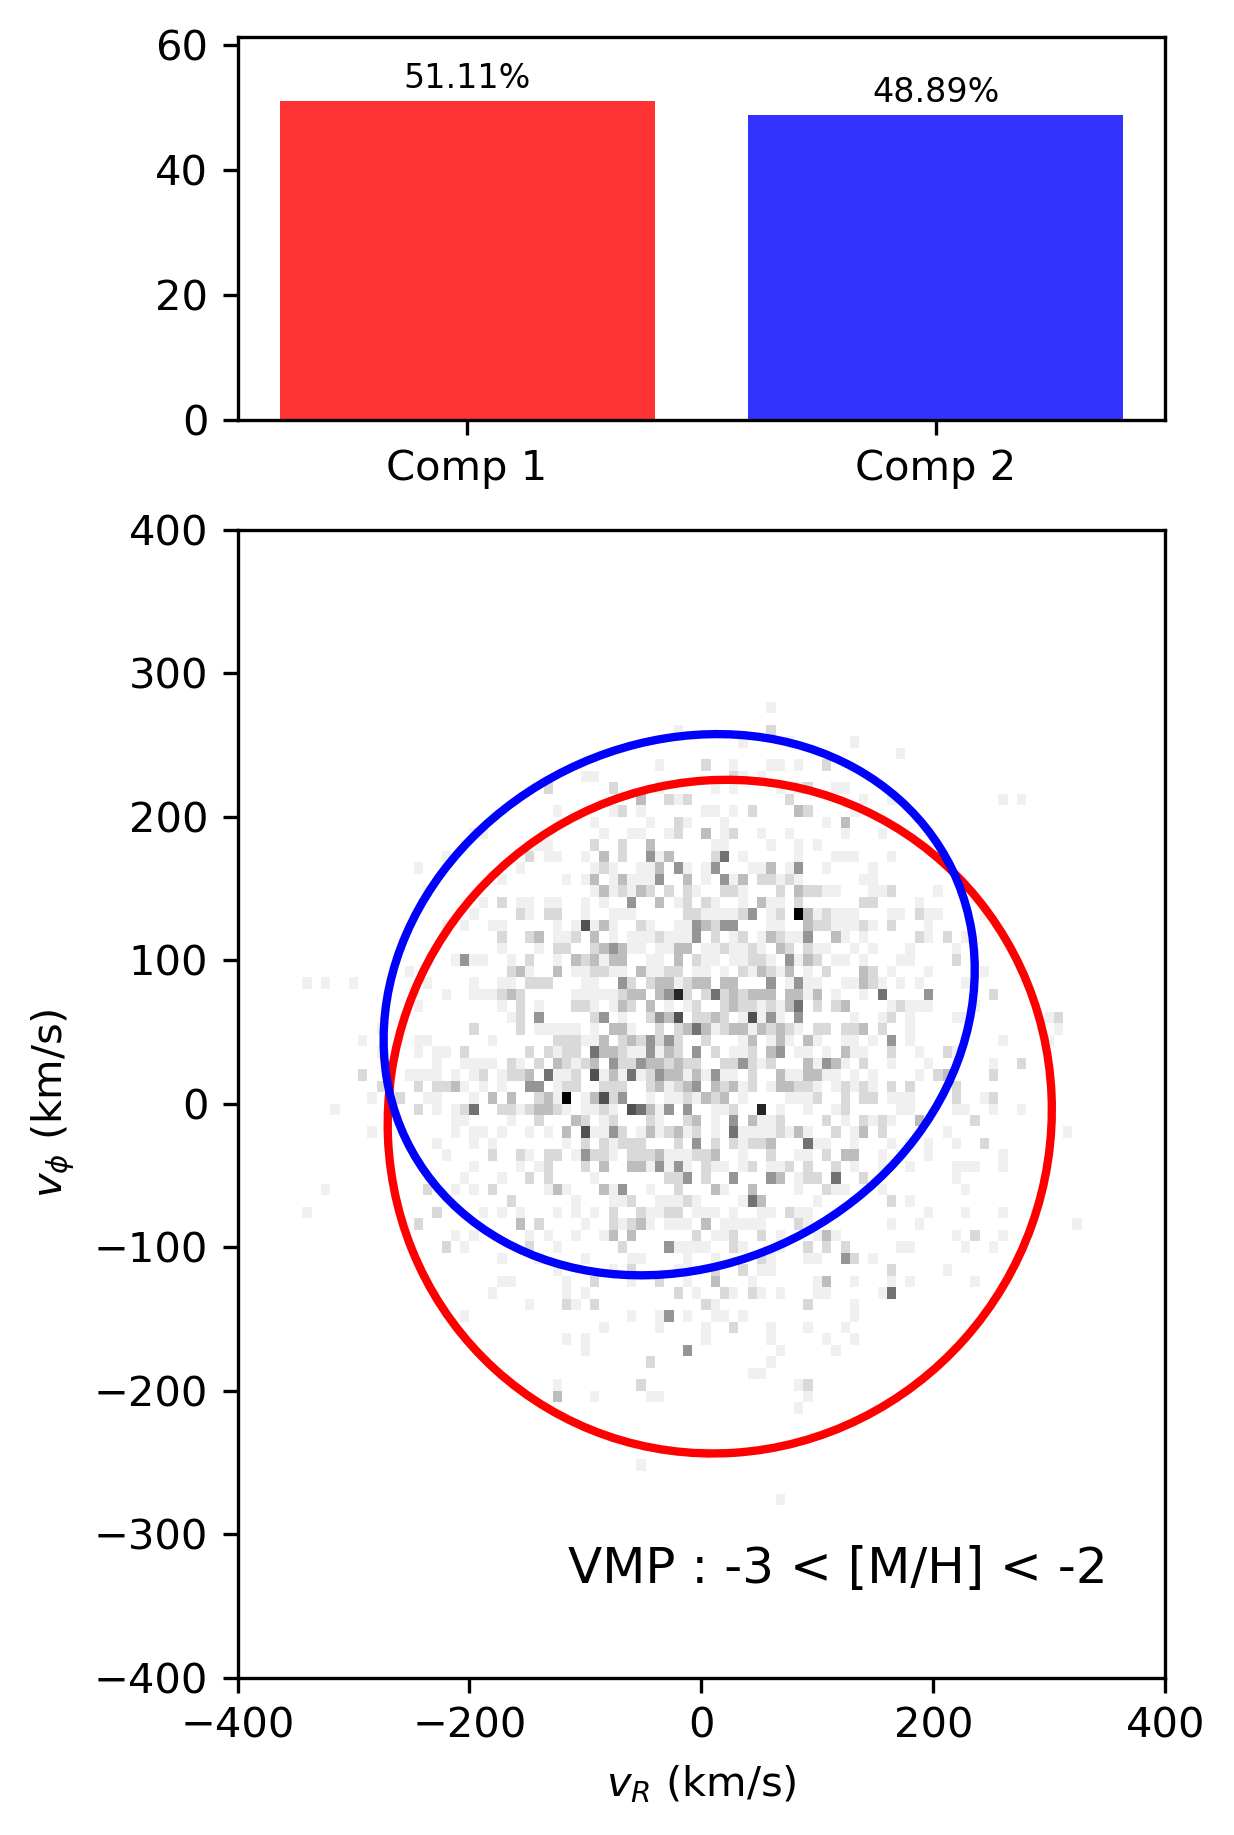
\includegraphics[width=\linewidth]{../figures/gmm_VMP.png}
    \caption{\href{https://raw.githack.com/raunaq-rai/Disentangling-the-Milky-Way-using-GMM/main/figures/VMP\_\_-3\%5BM\_H\%5D-2.html}{VMP}}
    \label{fig:gmm_vmp}
  \end{subfigure}\hfill
  \begin{subfigure}[t]{0.24\linewidth}
    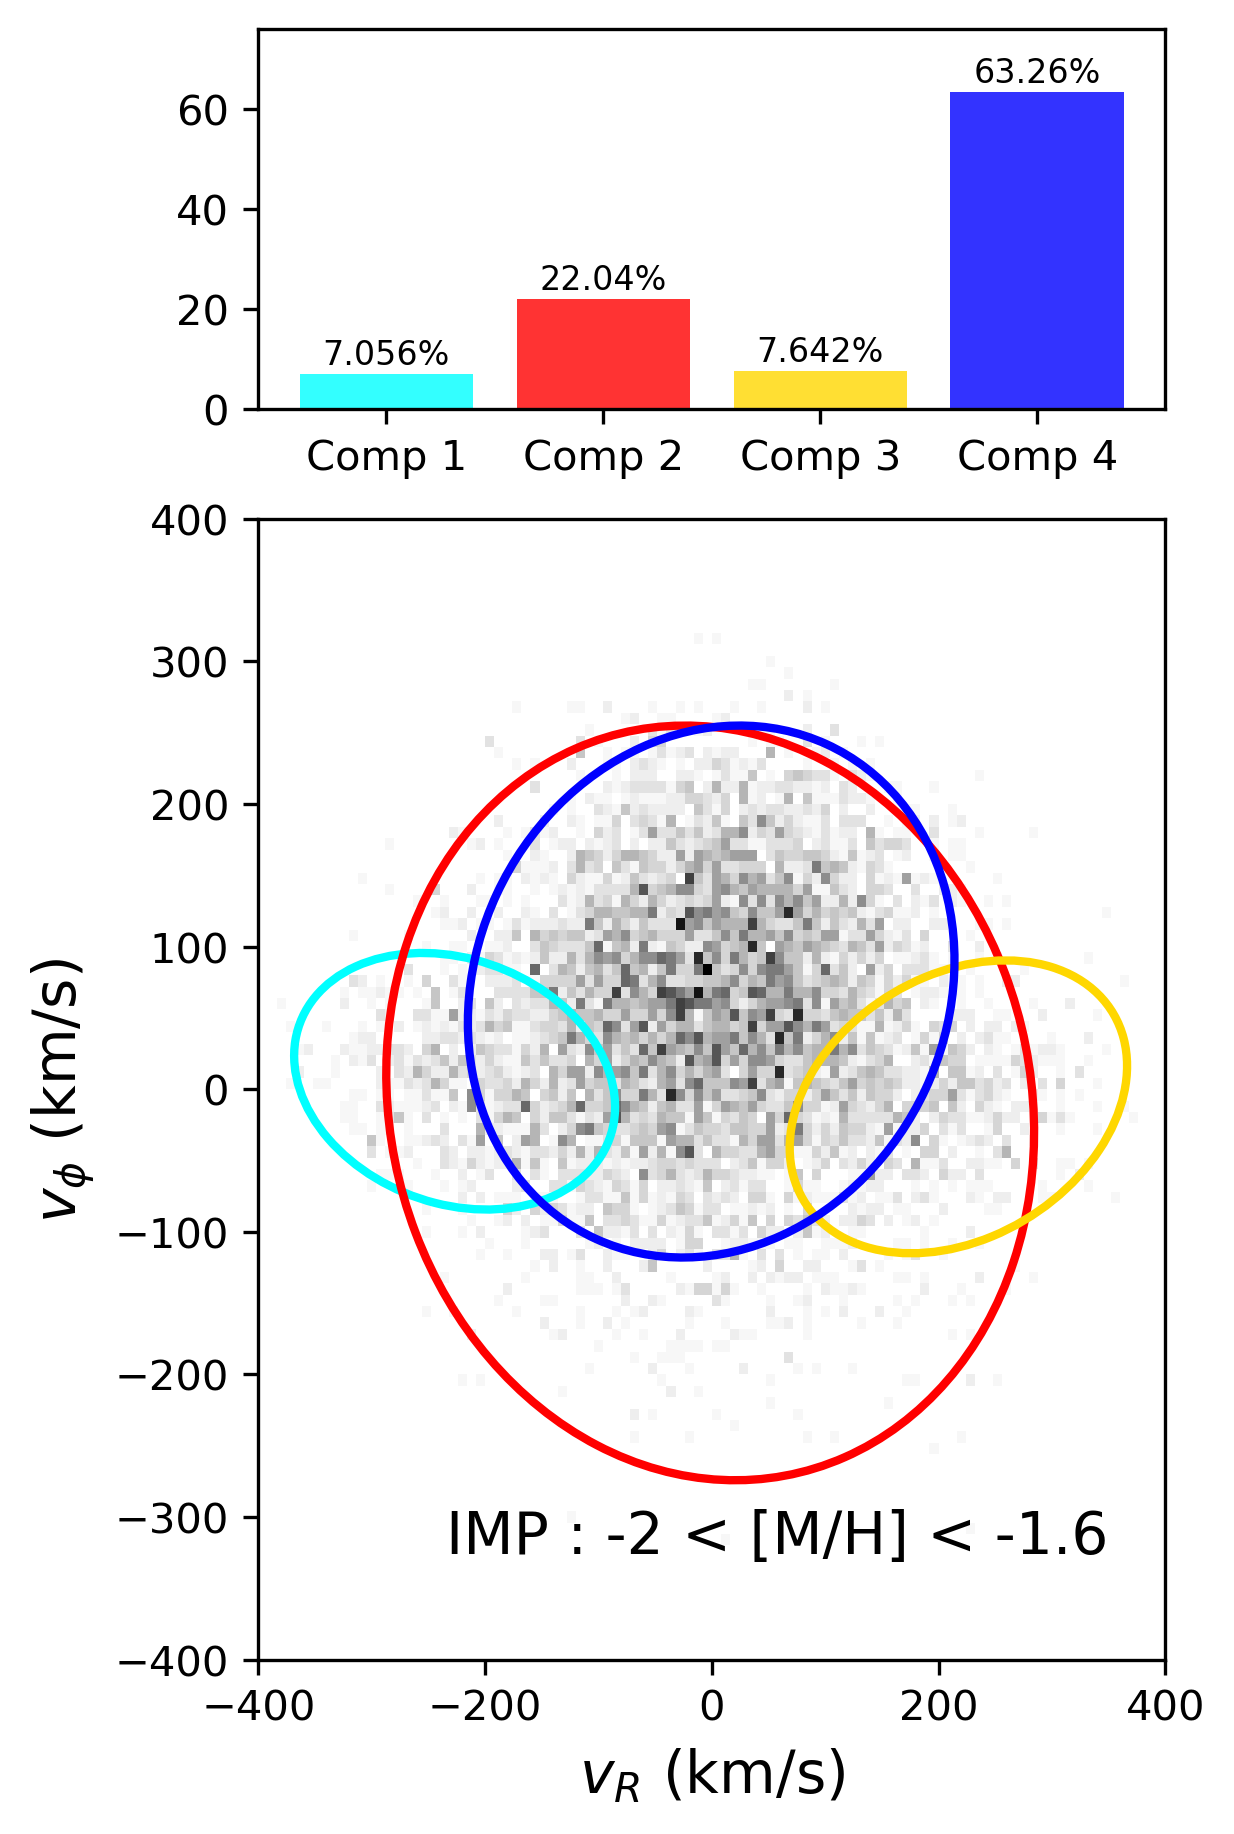
\includegraphics[width=\linewidth]{../figures/gmm_IMP.png}
    \caption{\href{https://raw.githack.com/raunaq-rai/Disentangling-the-Milky-Way-using-GMM/main/figures/IMP\_\_-2\%5BM\_H\%5D-1.6.html}{IMP}}
    \label{fig:gmm_imp}
  \end{subfigure}\hfill
  \begin{subfigure}[t]{0.24\linewidth}
    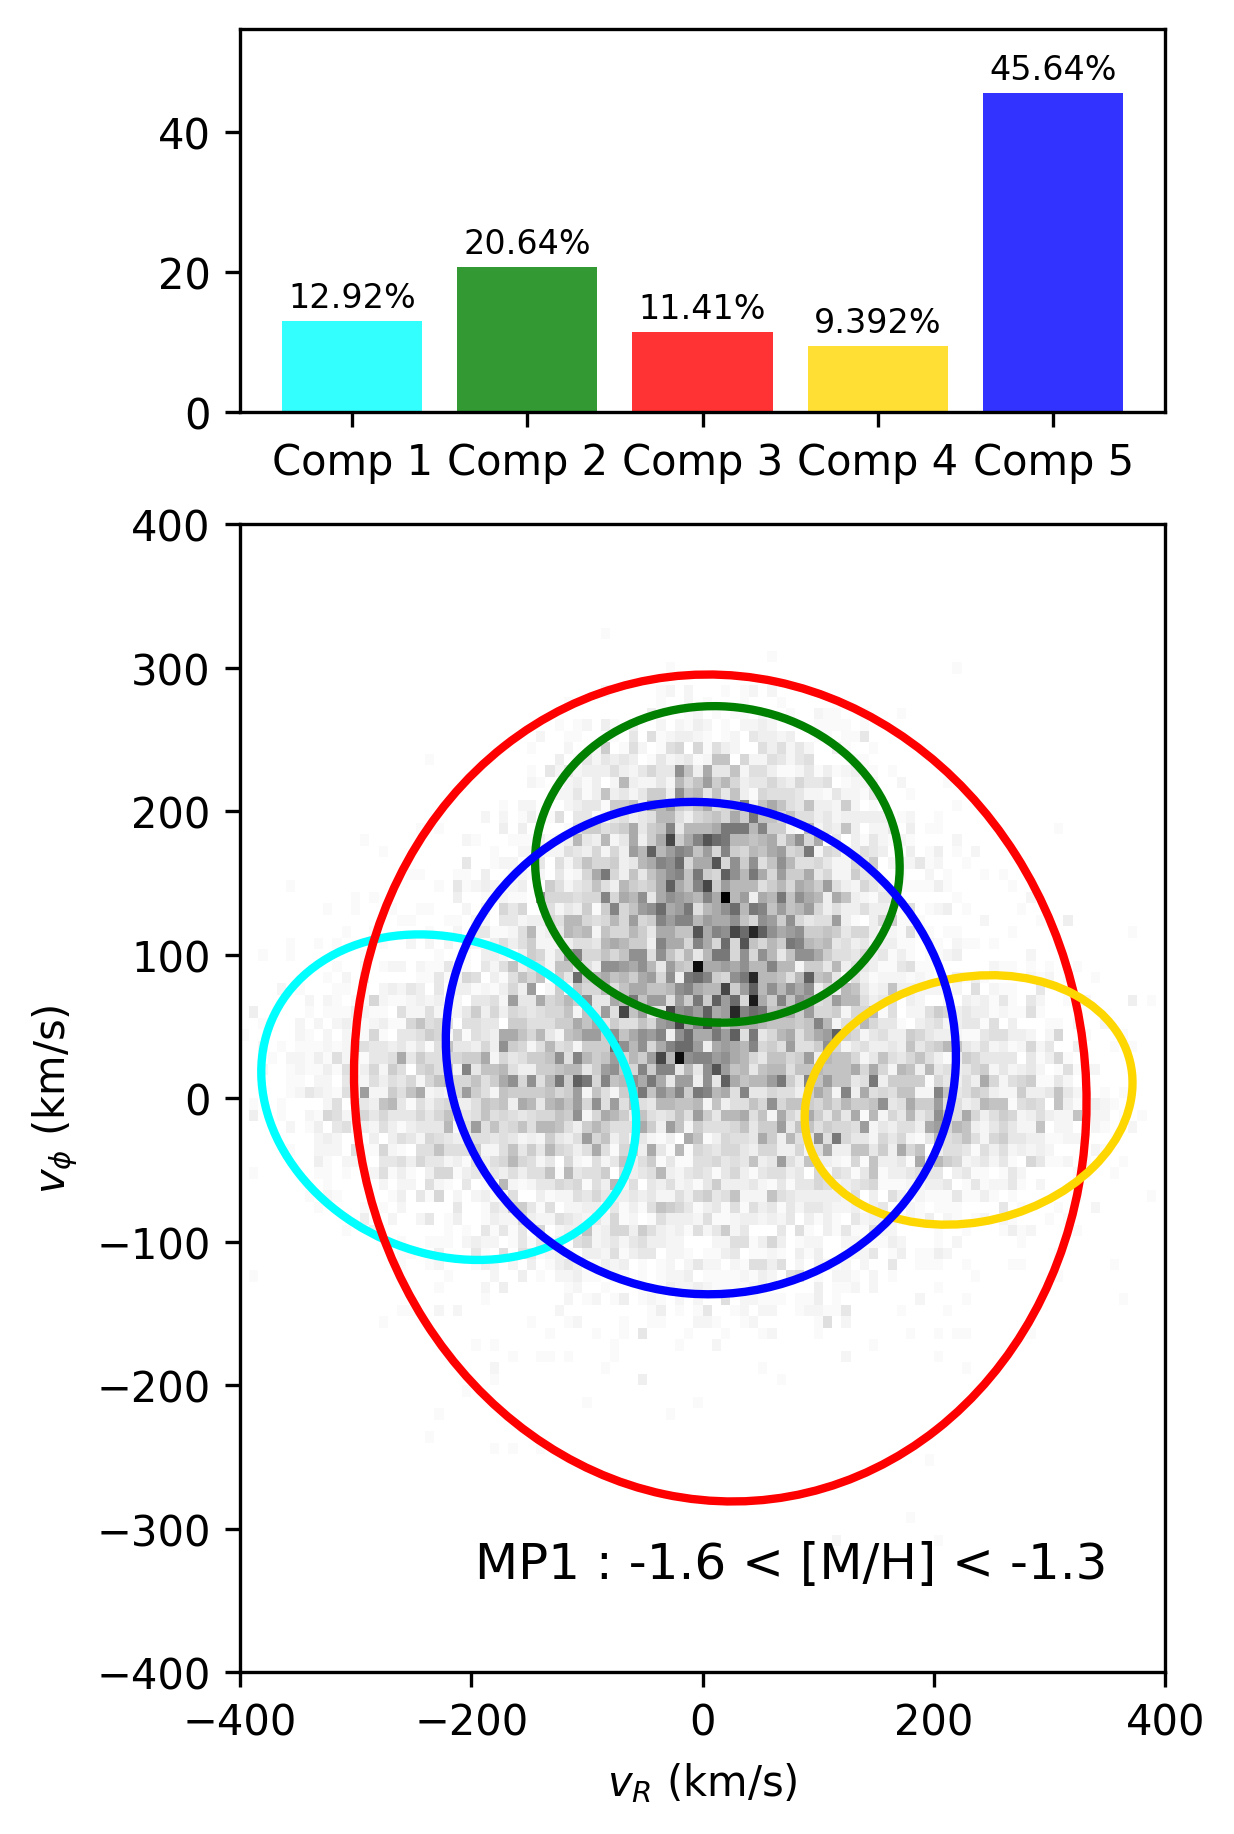
\includegraphics[width=\linewidth]{../figures/gmm_MP1.png}
    \caption{\href{https://raw.githack.com/raunaq-rai/Disentangling-the-Milky-Way-using-GMM/main/figures/MP1\_\_-1.6\%5BM\_H\%5D-1.3.html}{MP1}}
    \label{fig:gmm_mp1}
  \end{subfigure}\hfill
  \begin{subfigure}[t]{0.24\linewidth}
    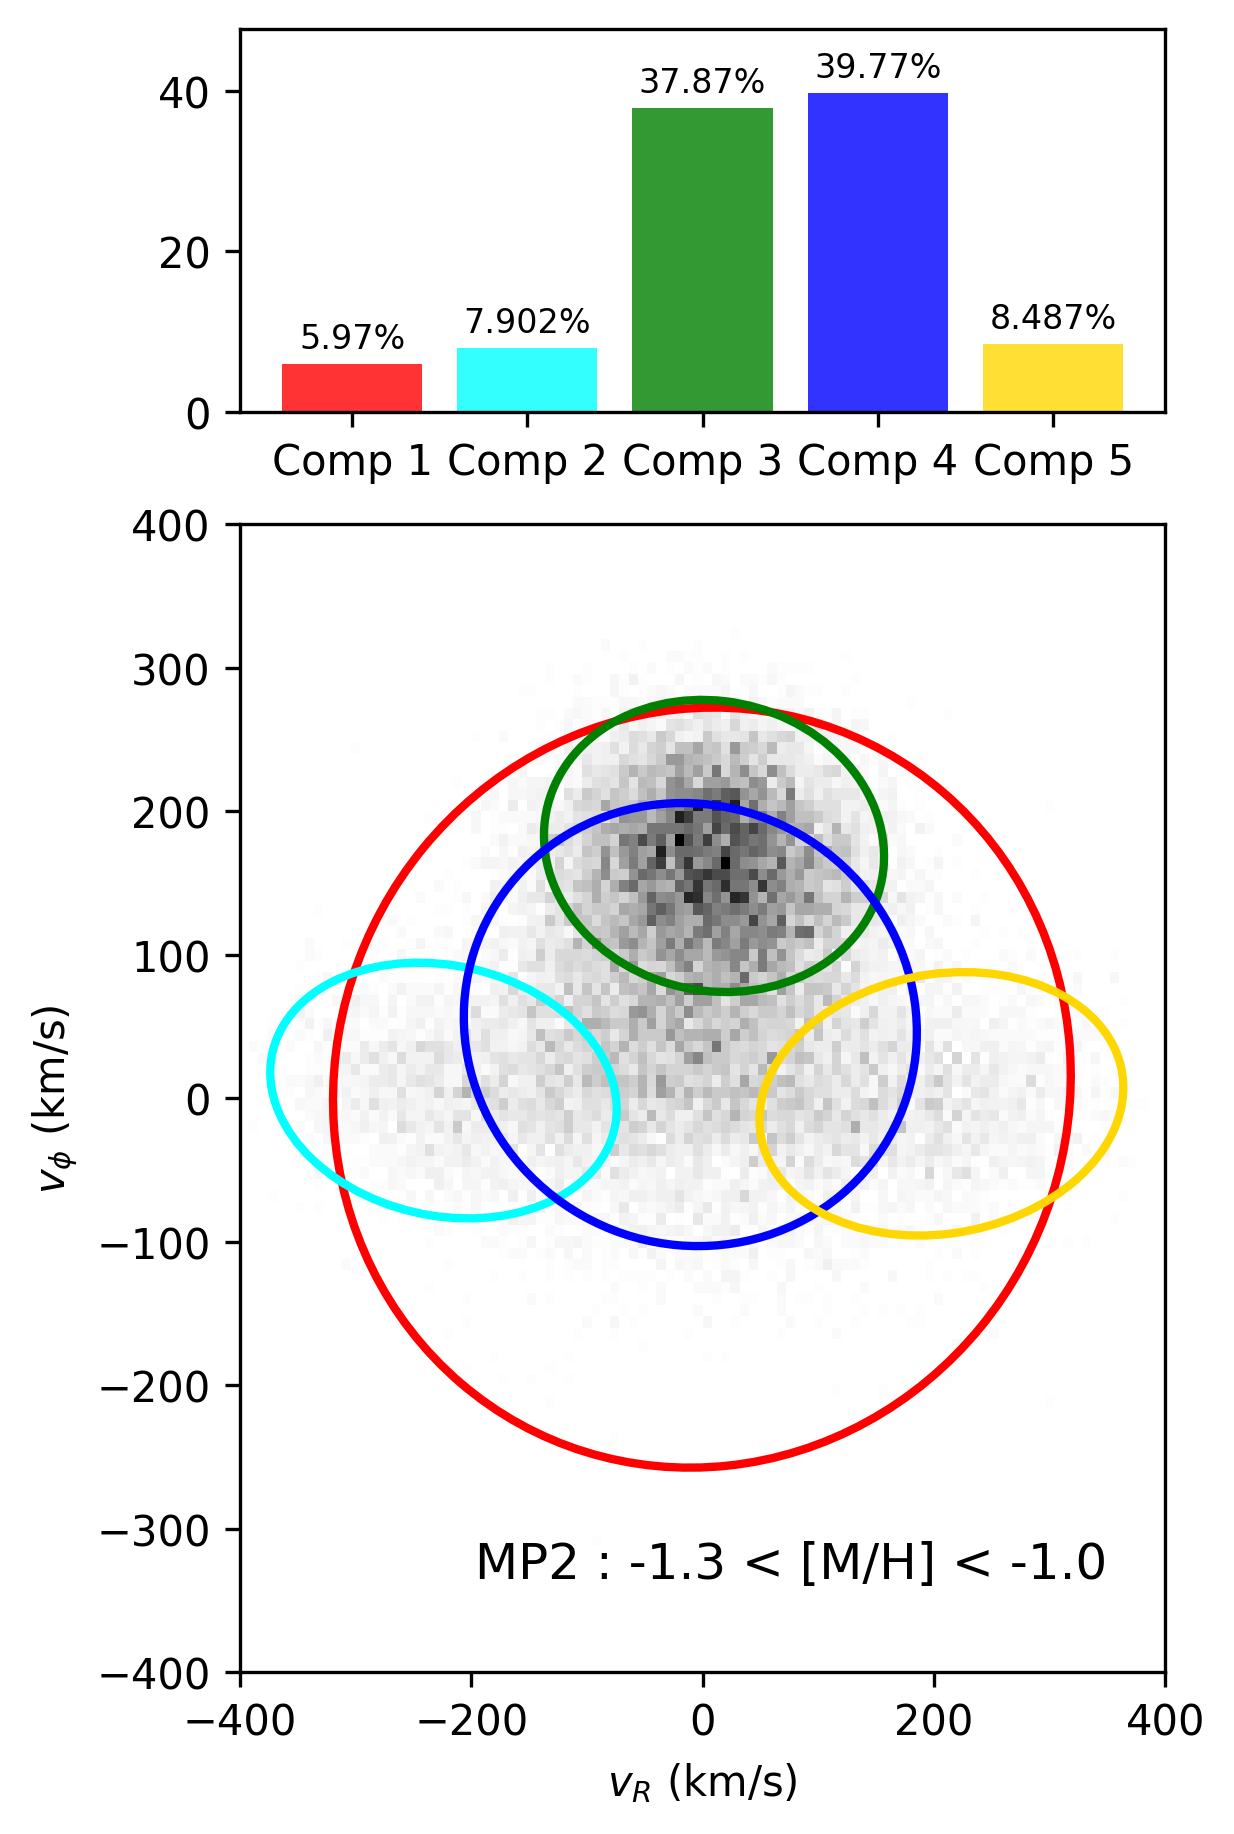
\includegraphics[width=\linewidth]{../figures/gmm_MP2.png}
    \caption{\href{https://raw.githack.com/raunaq-rai/Disentangling-the-Milky-Way-using-GMM/main/figures/MP2\_\_-1.3\%5BM\_H\%5D-1.0.html}{MP2}}
    \label{fig:gmm_mp2}
  \end{subfigure}

  \caption{XD-GMM decomposition of red giant kinematics across metallicity bins. Links to the fully interactive 3-D plots for each bin are provided in the subcaptions.}
  \label{fig:gmm_zhang}
\end{figure}

\paragraph{1. No metal-poor disc.}
Below $\mathrm{[M/H]}\lesssim-2$ we find \textbf{only halo kinematics}: one
nearly stationary Gaussian and a mildly prograde “Aurora” halo
component~\cite{Belokurov2022}.  Monte-Carlo residual tests place a strict
upper limit of $<1\%$ on any hidden, rotation-supported disc in this regime.

\paragraph{2. Onset of the thick disc.}
Disc-like rotation emerges at $\mathrm{[M/H]}\gtrsim-1.6$ as a thick-disc
Gaussian containing $\sim22\%$ of stars and
$V_{\rm rot}/\sigma_\phi\!\approx\!2.8$.  By
$\mathrm{[M/H]}\approx-1.3$ the component grows to $\sim37\%$ and exceeds the
canonical “discy” threshold with $V_{\rm rot}/\sigma_\phi\!\approx\!3.5$.



\paragraph{3. Chemistry splits the timeline.(Fig.~\ref{fig:mh_vphi_alpha}).}
\begin{itemize}
  \item \textit{High-$\alpha$ branch:} rotation support rises gradually from
        $\mathrm{[M/H]}\!\sim\!-2$ to $-1$, indicating an early, steady build-up
        of the thick disc.
  \item \textit{Low-$\alpha$ branch:} remains dispersion-dominated until a
        sharp spin-up at $\mathrm{[M/H]}\!\sim\!-1.3$, marking a later, more
        rapid disc formation episode.
\end{itemize}

\begin{figure}[H]
  \centering
  \begin{subfigure}[t]{0.48\linewidth}
    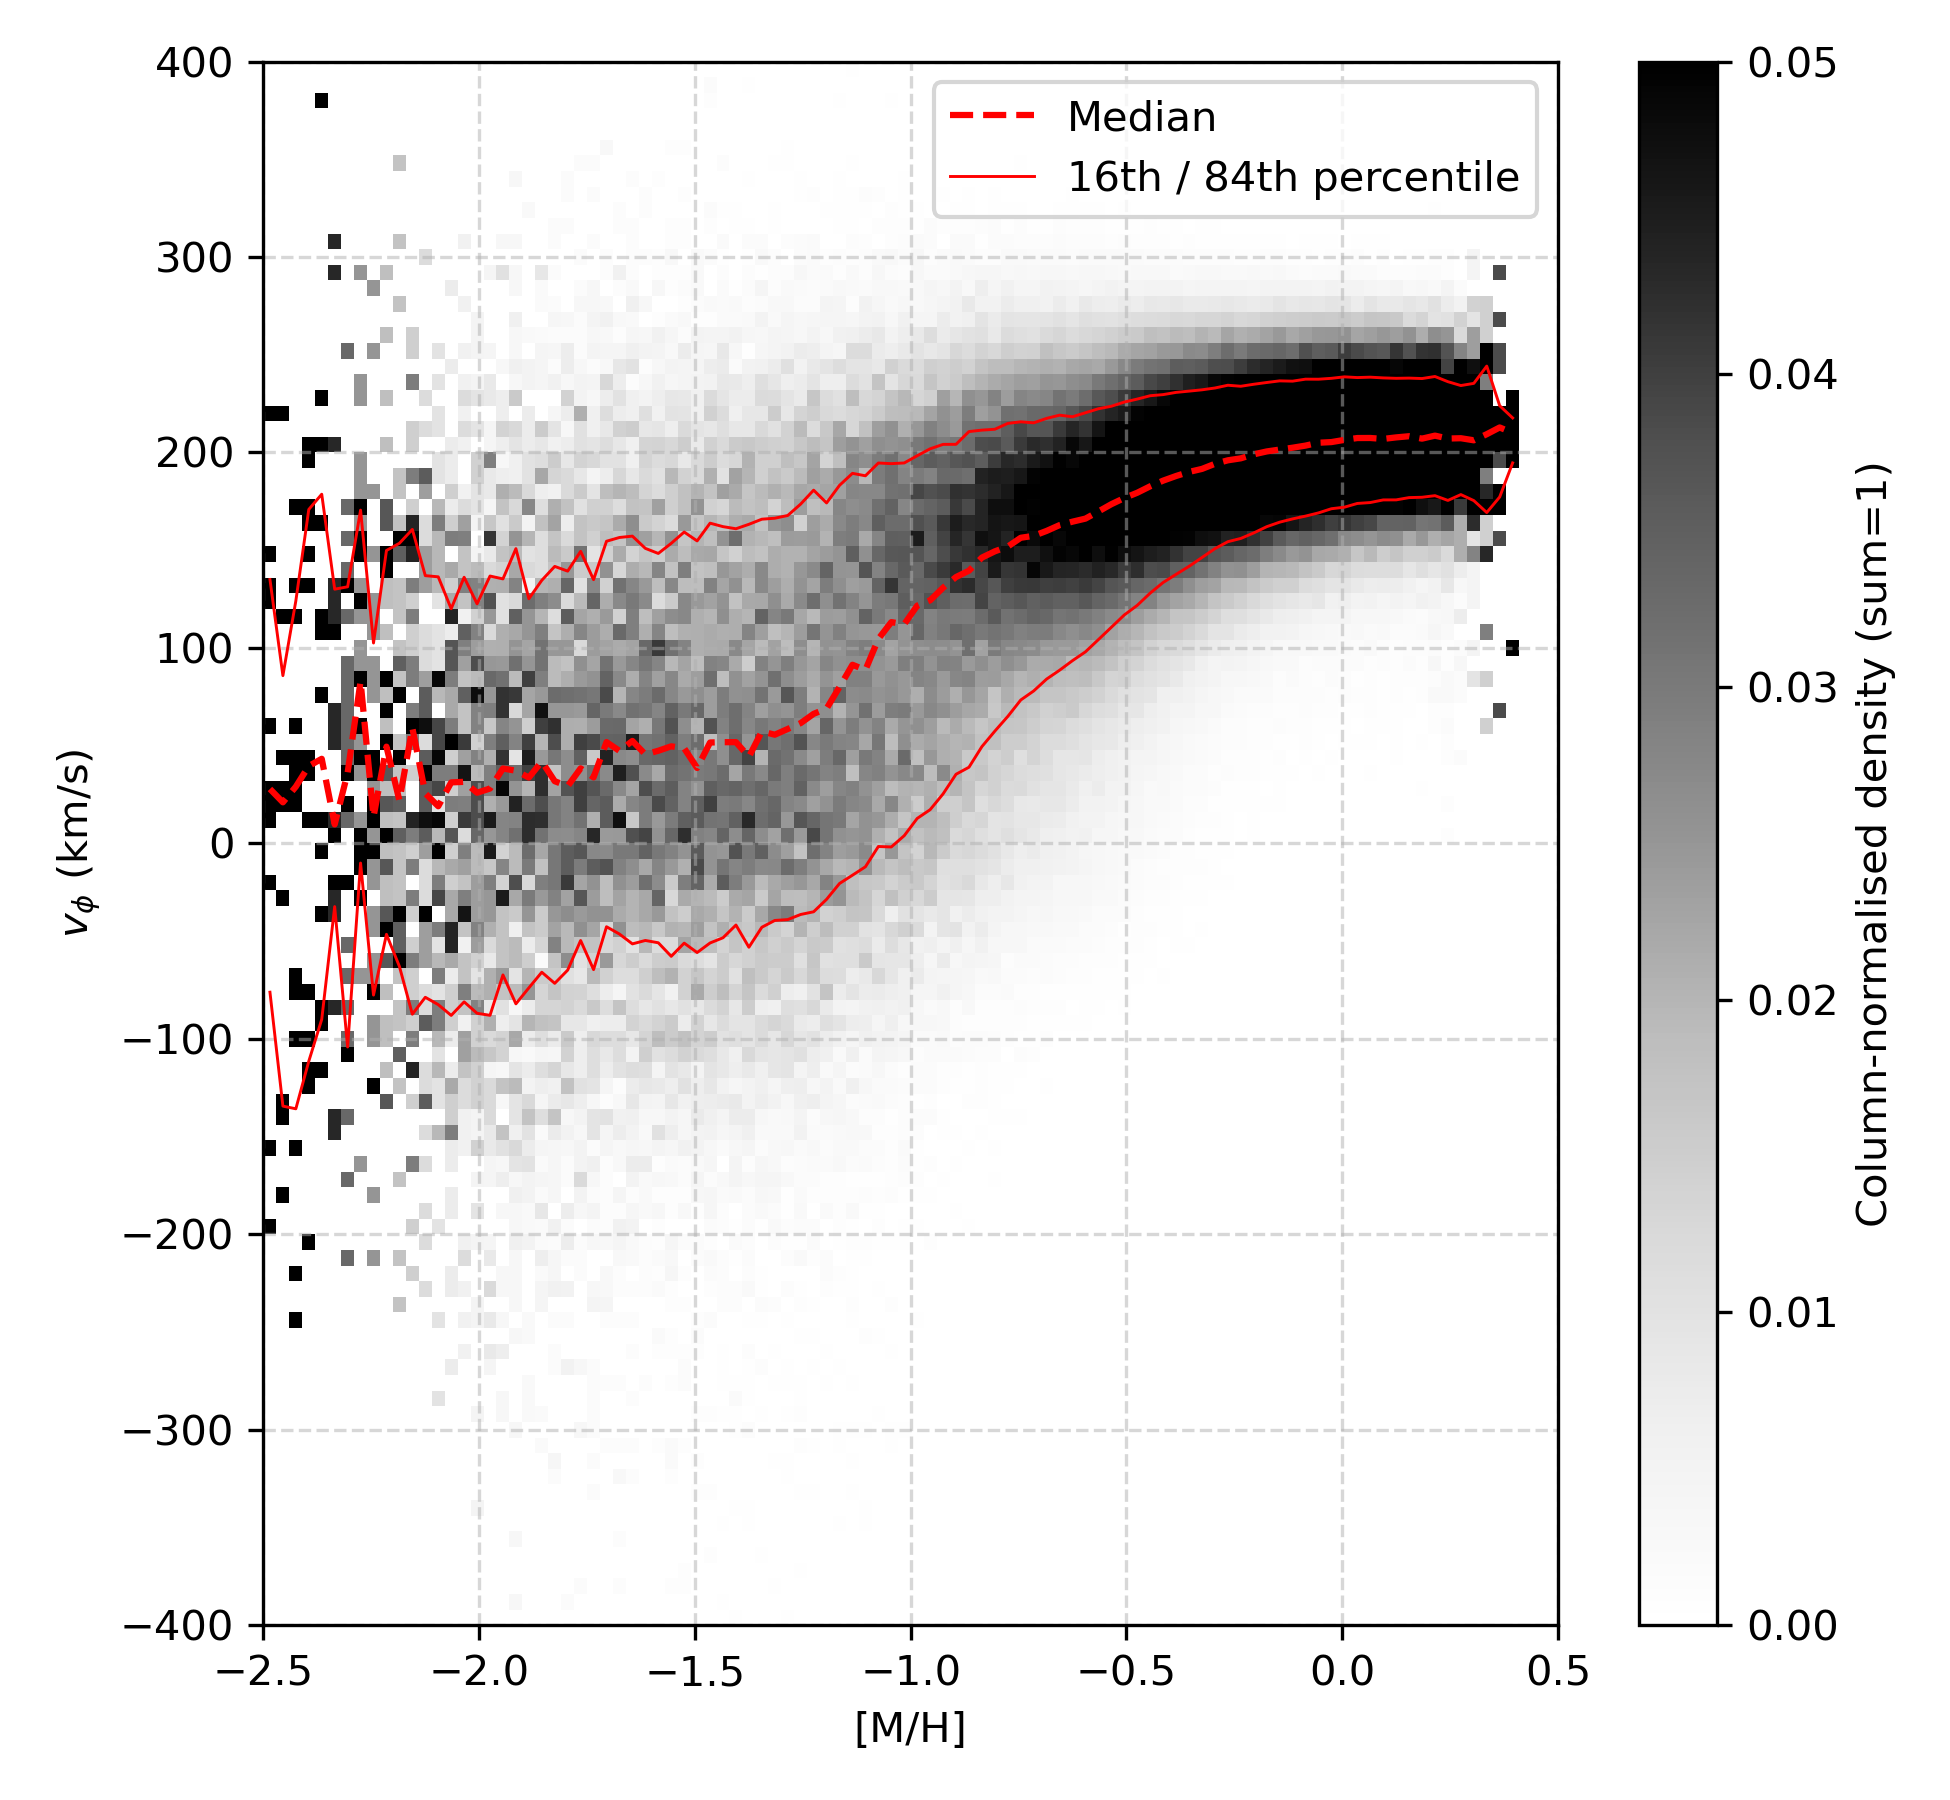
\includegraphics[width=\linewidth]{../figures/vis_mh_vphi_high_alpha.png}
    \caption{High $\alpha$ stars}
  \end{subfigure}
  \hfill
  \begin{subfigure}[t]{0.48\linewidth}
    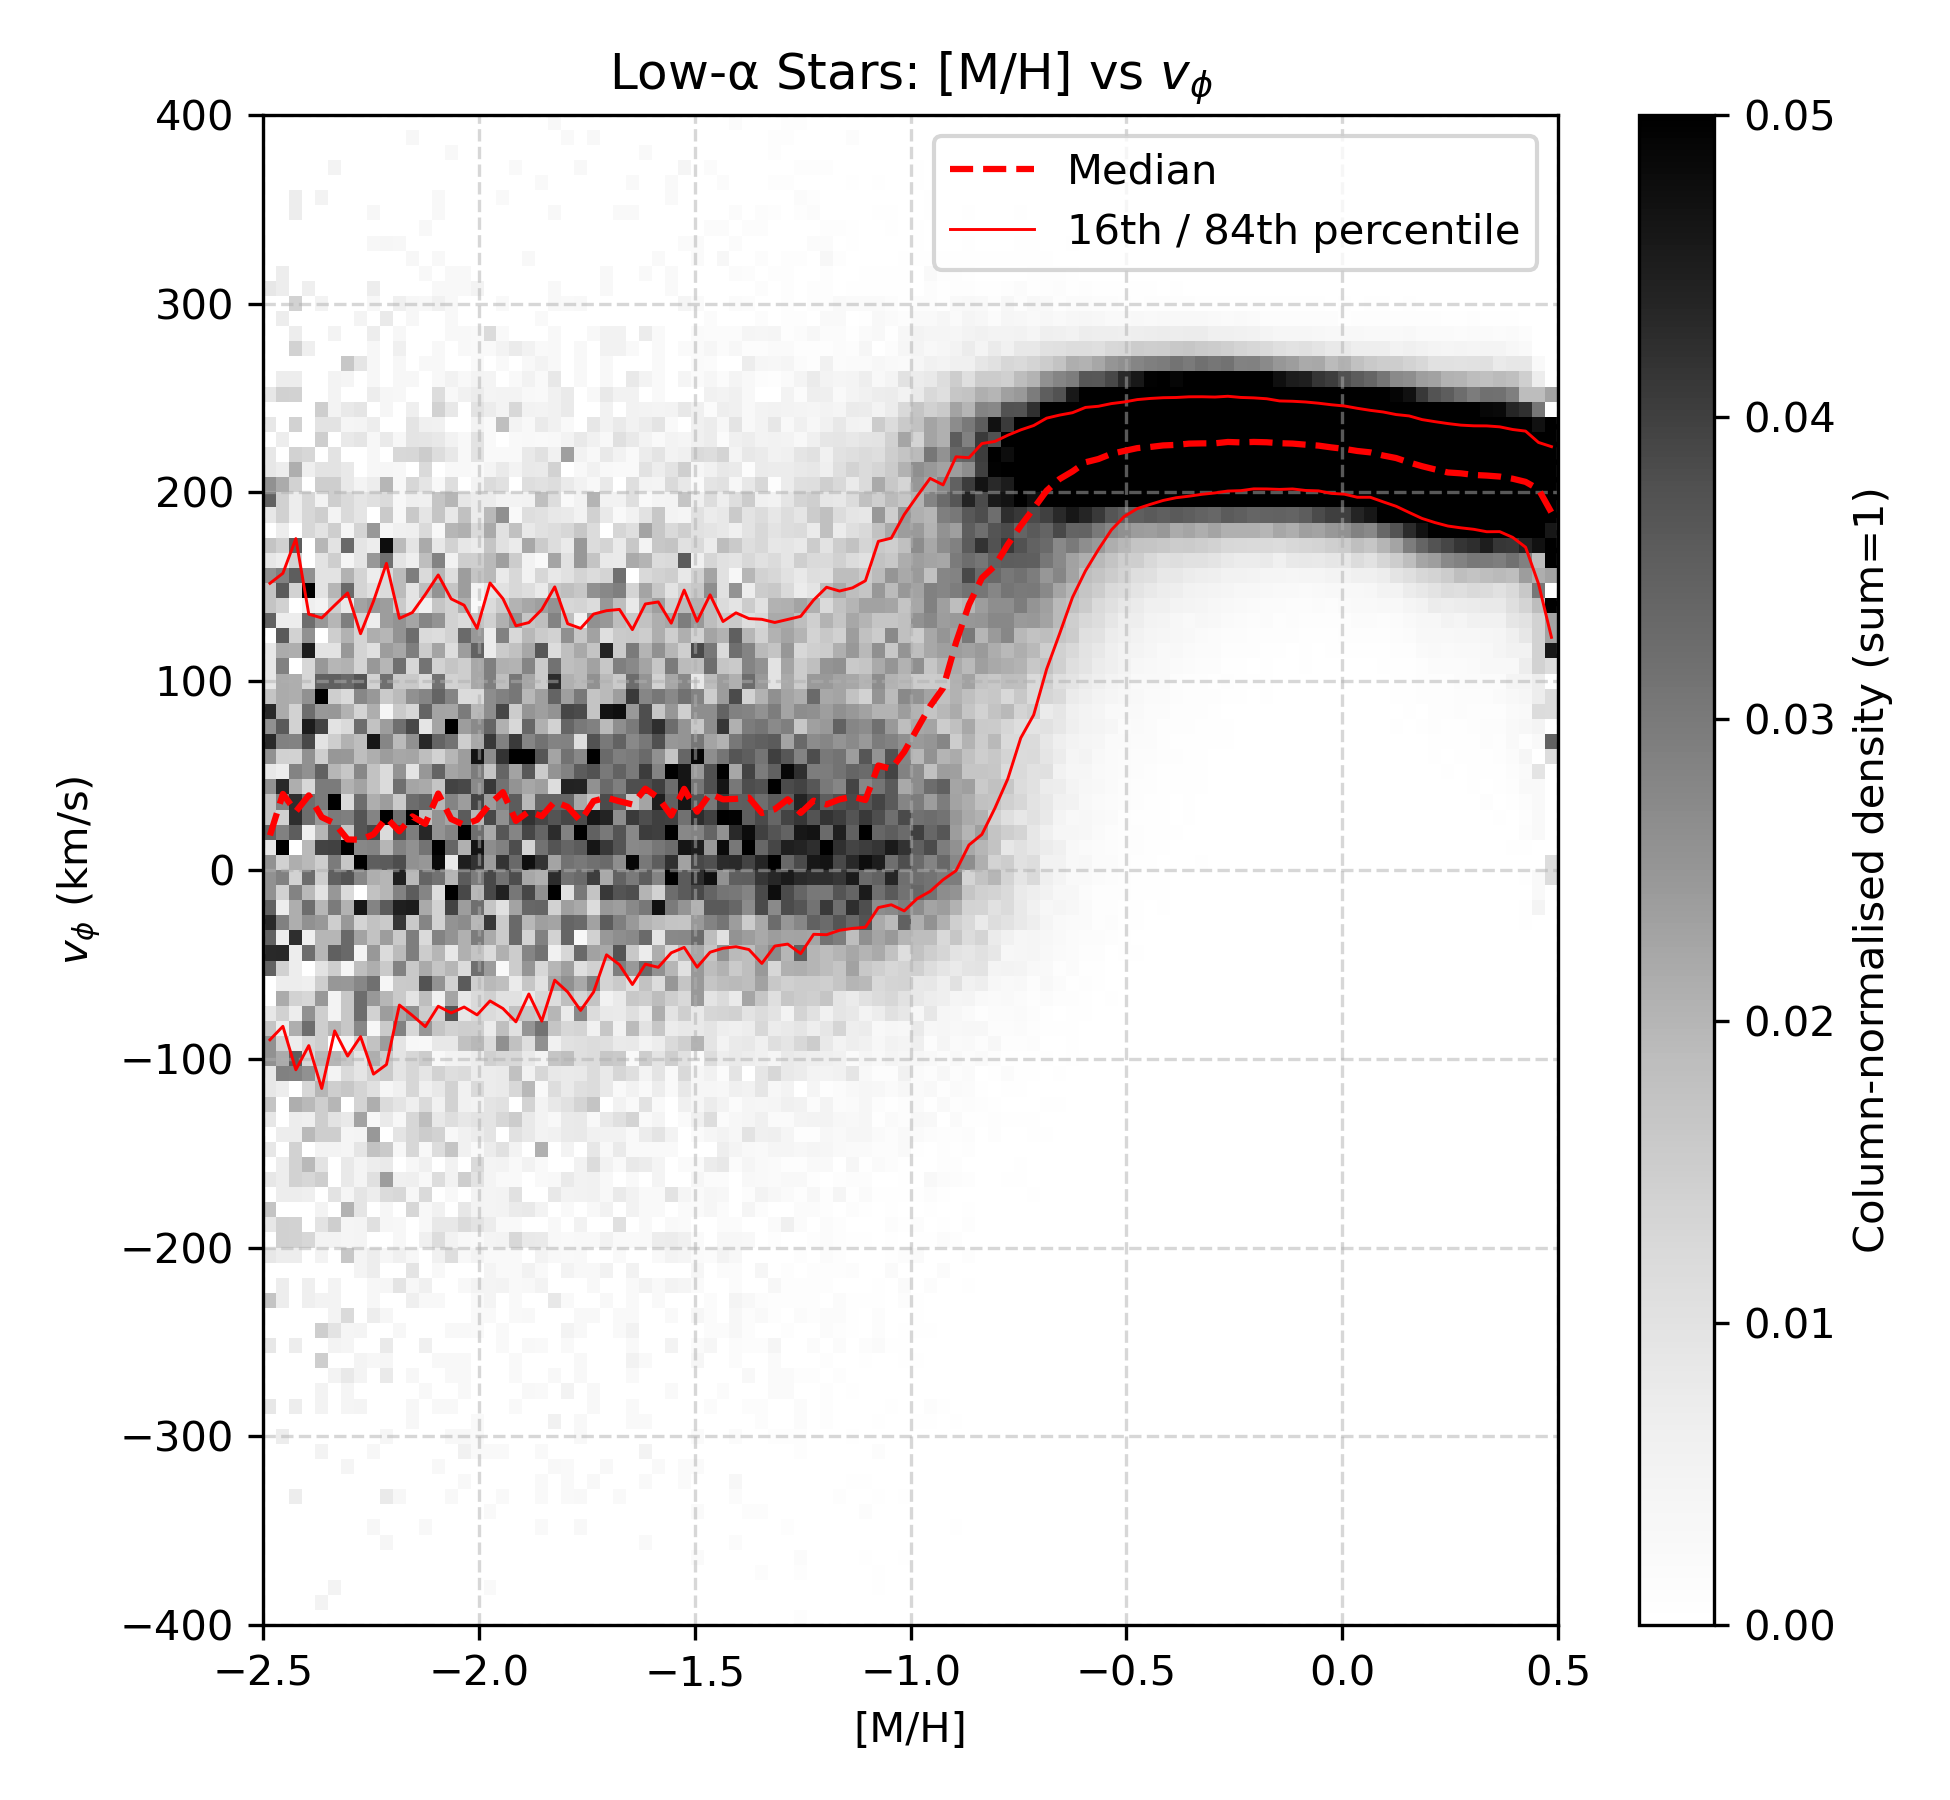
\includegraphics[width=\linewidth]{../figures/vis_mh_vphi_low_alpha.png}
    \caption{Low $\alpha$ stars}
  \end{subfigure}
  \caption{Median $v_\phi$ and dispersion vs.\ metallicity, split by $\alpha$-sequence.}
  \label{fig:mh_vphi_alpha}
\end{figure}

\begin{figure}[H]
  \centering
  % Row 1
  \begin{subfigure}[t]{0.24\linewidth}
    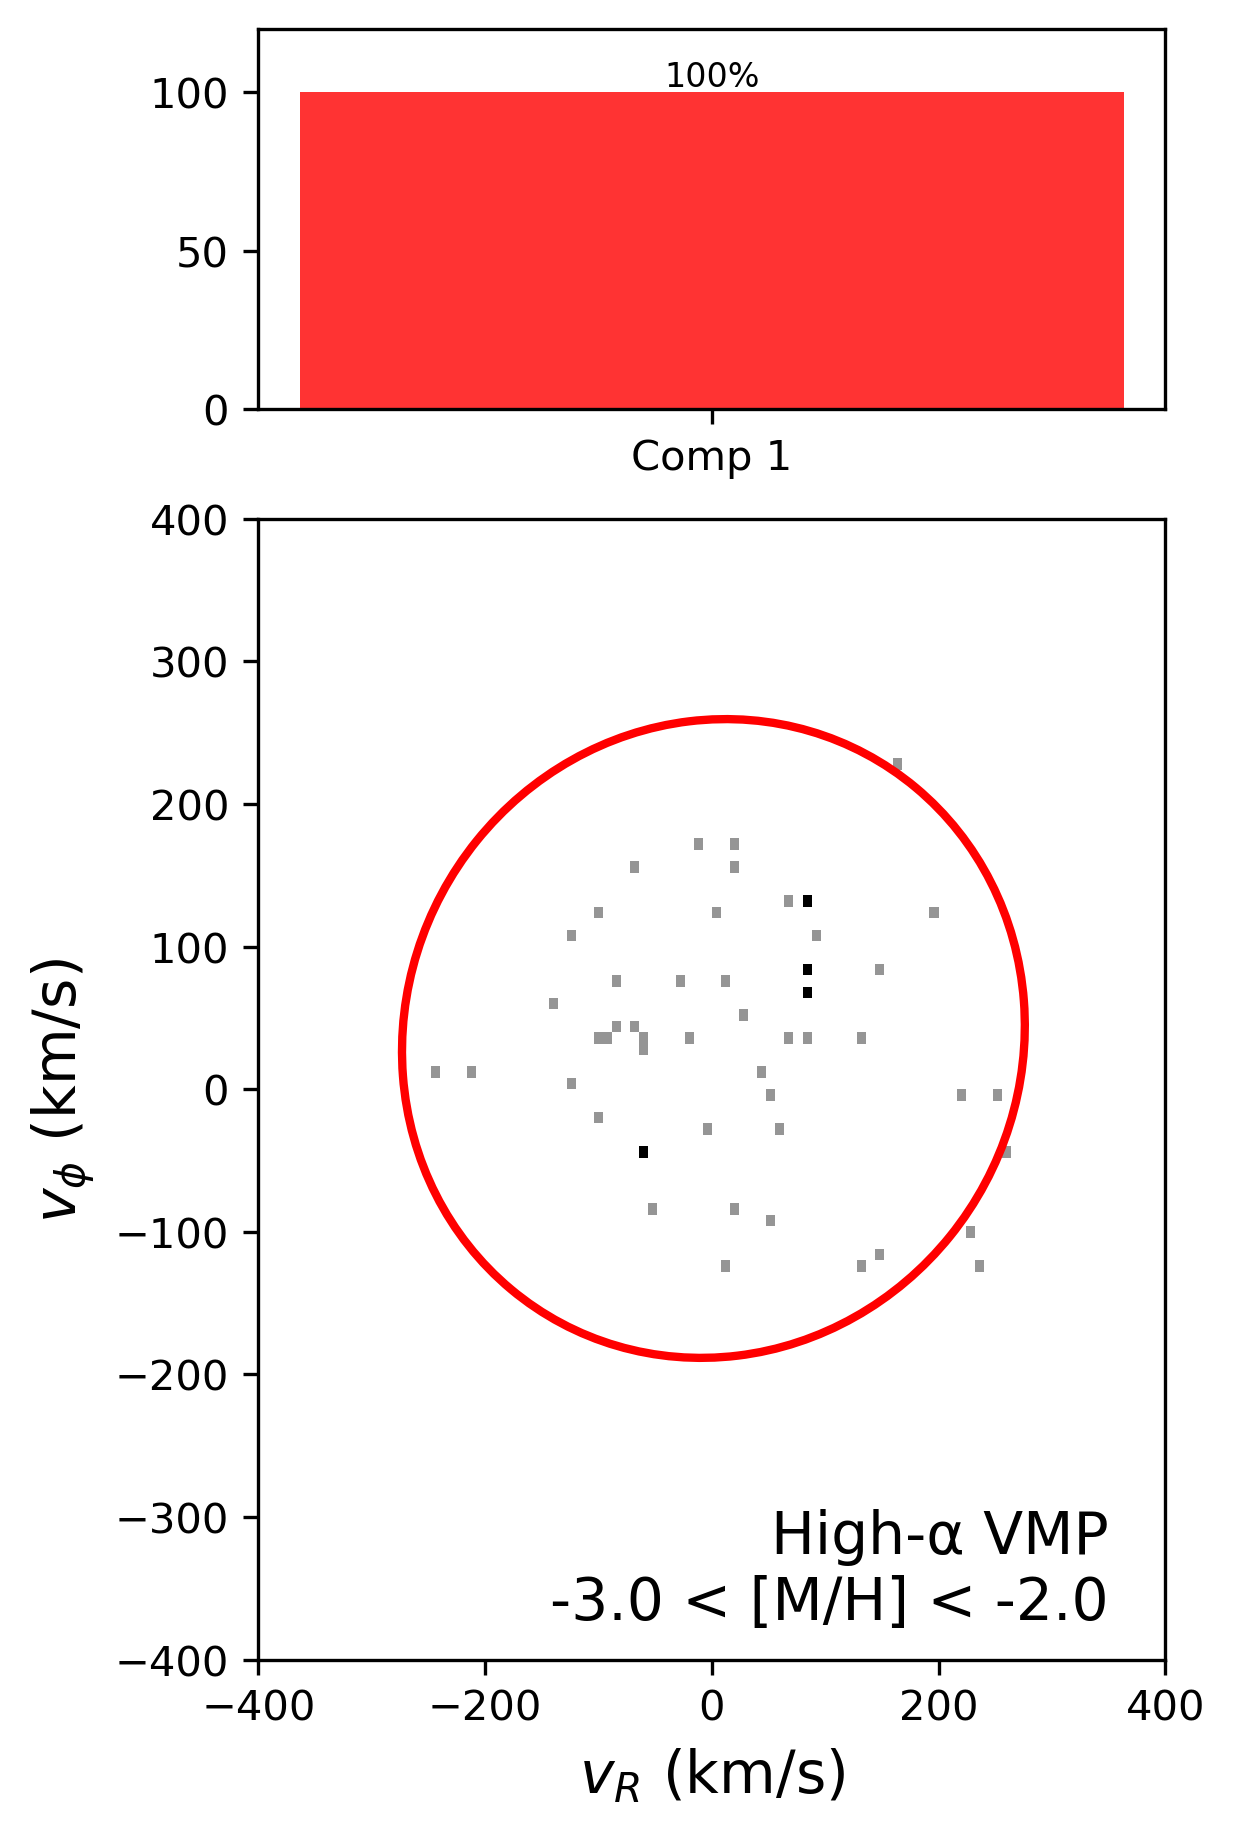
\includegraphics[width=\linewidth]{../figures/gmm_vmp_high_alpha_k1.png}
    \caption{\href{https://raw.githack.com/raunaq-rai/Disentangling-the-Milky-Way-using-GMM/main/figures/VMP\_high\_\_\_-3\%5BM\_H\%5D-2.html}{VMP $\alpha_{\mathrm{high}}$}}
    \label{fig:vmp_hi}
  \end{subfigure}\hfill
  \begin{subfigure}[t]{0.24\linewidth}
    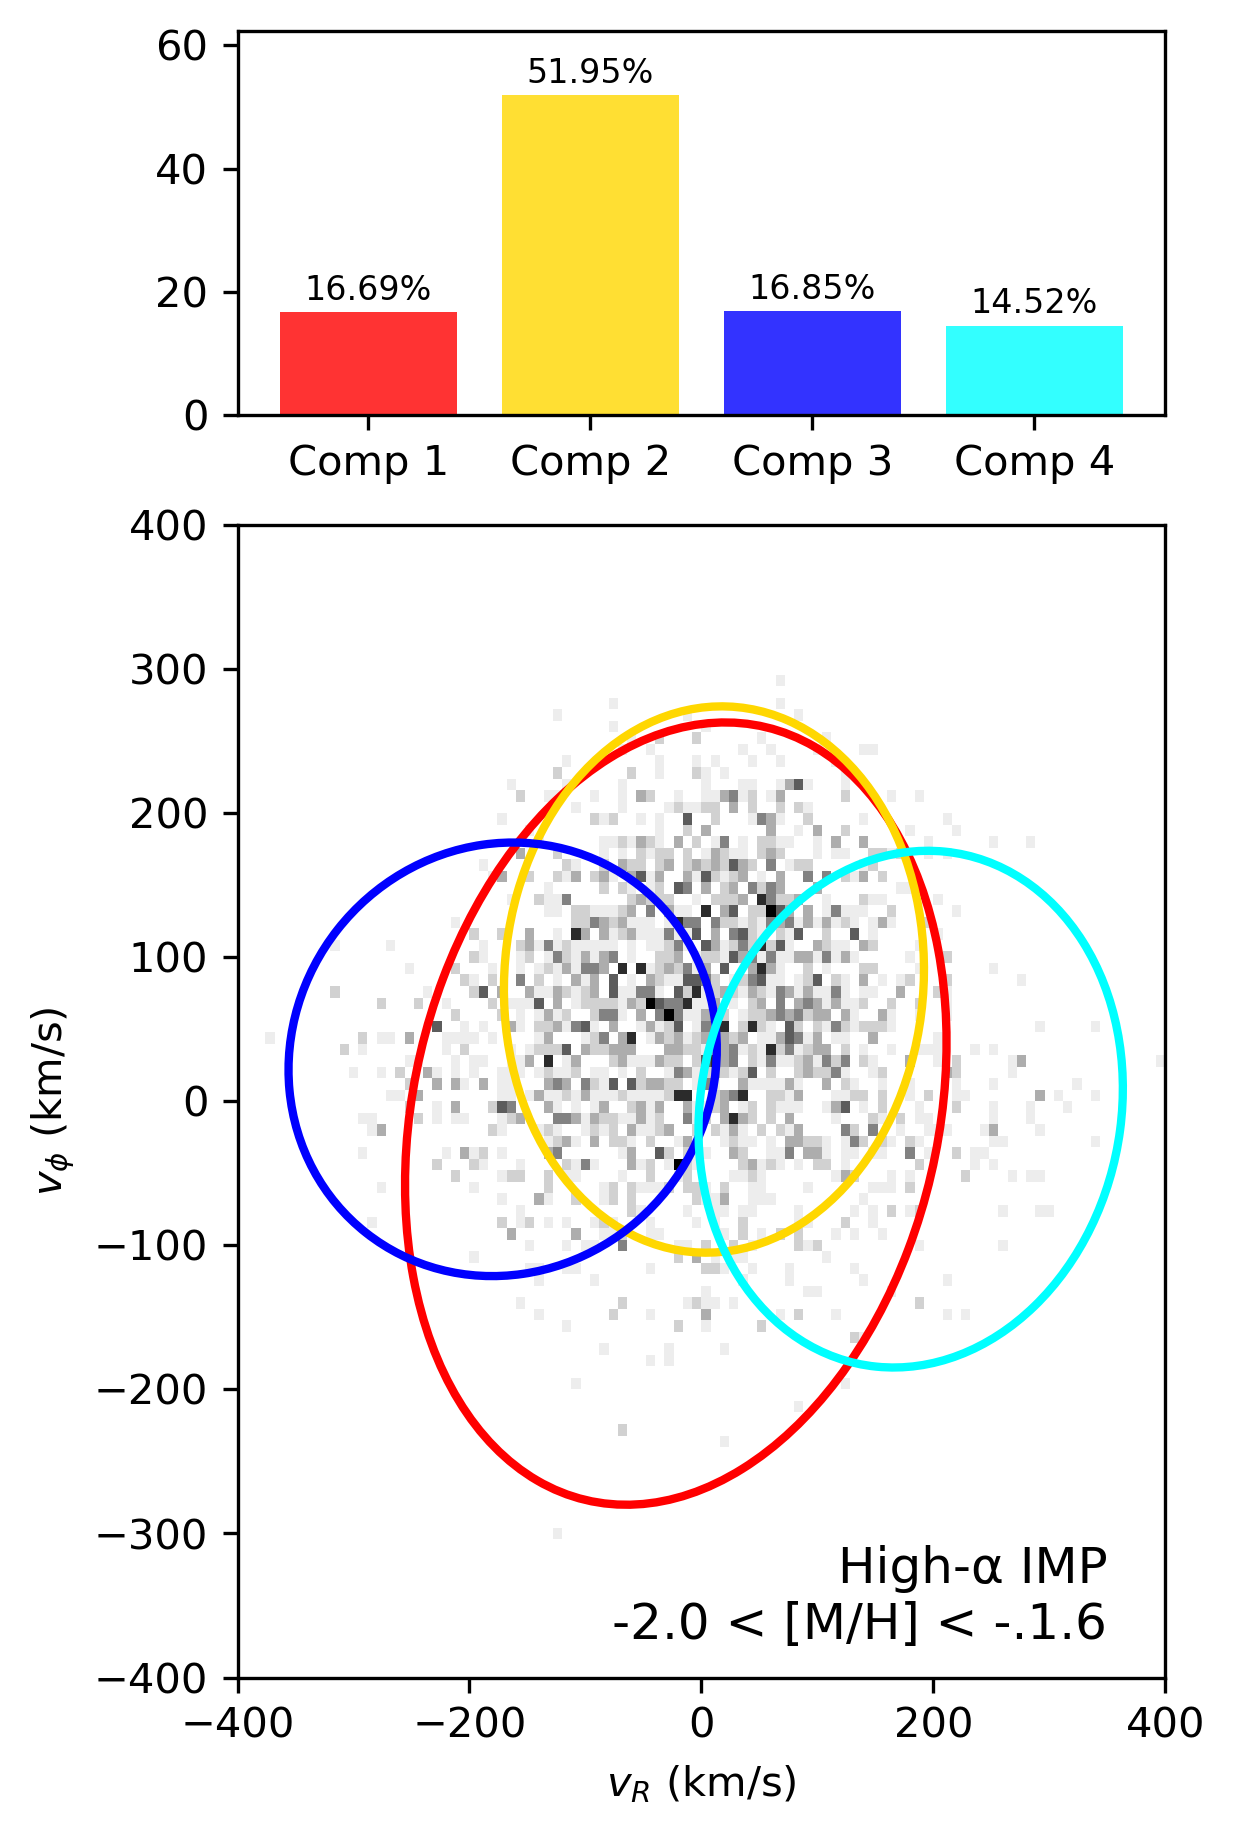
\includegraphics[width=\linewidth]{../figures/gmm_imp_high_alpha_k4.png}
    \caption{\href{https://raw.githack.com/raunaq-rai/Disentangling-the-Milky-Way-using-GMM/main/figures/IMP\_high\_\_\_-2\%5BM\_H\%5D-1.6.html}{IMP $\alpha_{\mathrm{high}}$}}
    \label{fig:imp_hi}
  \end{subfigure}\hfill
  \begin{subfigure}[t]{0.24\linewidth}
    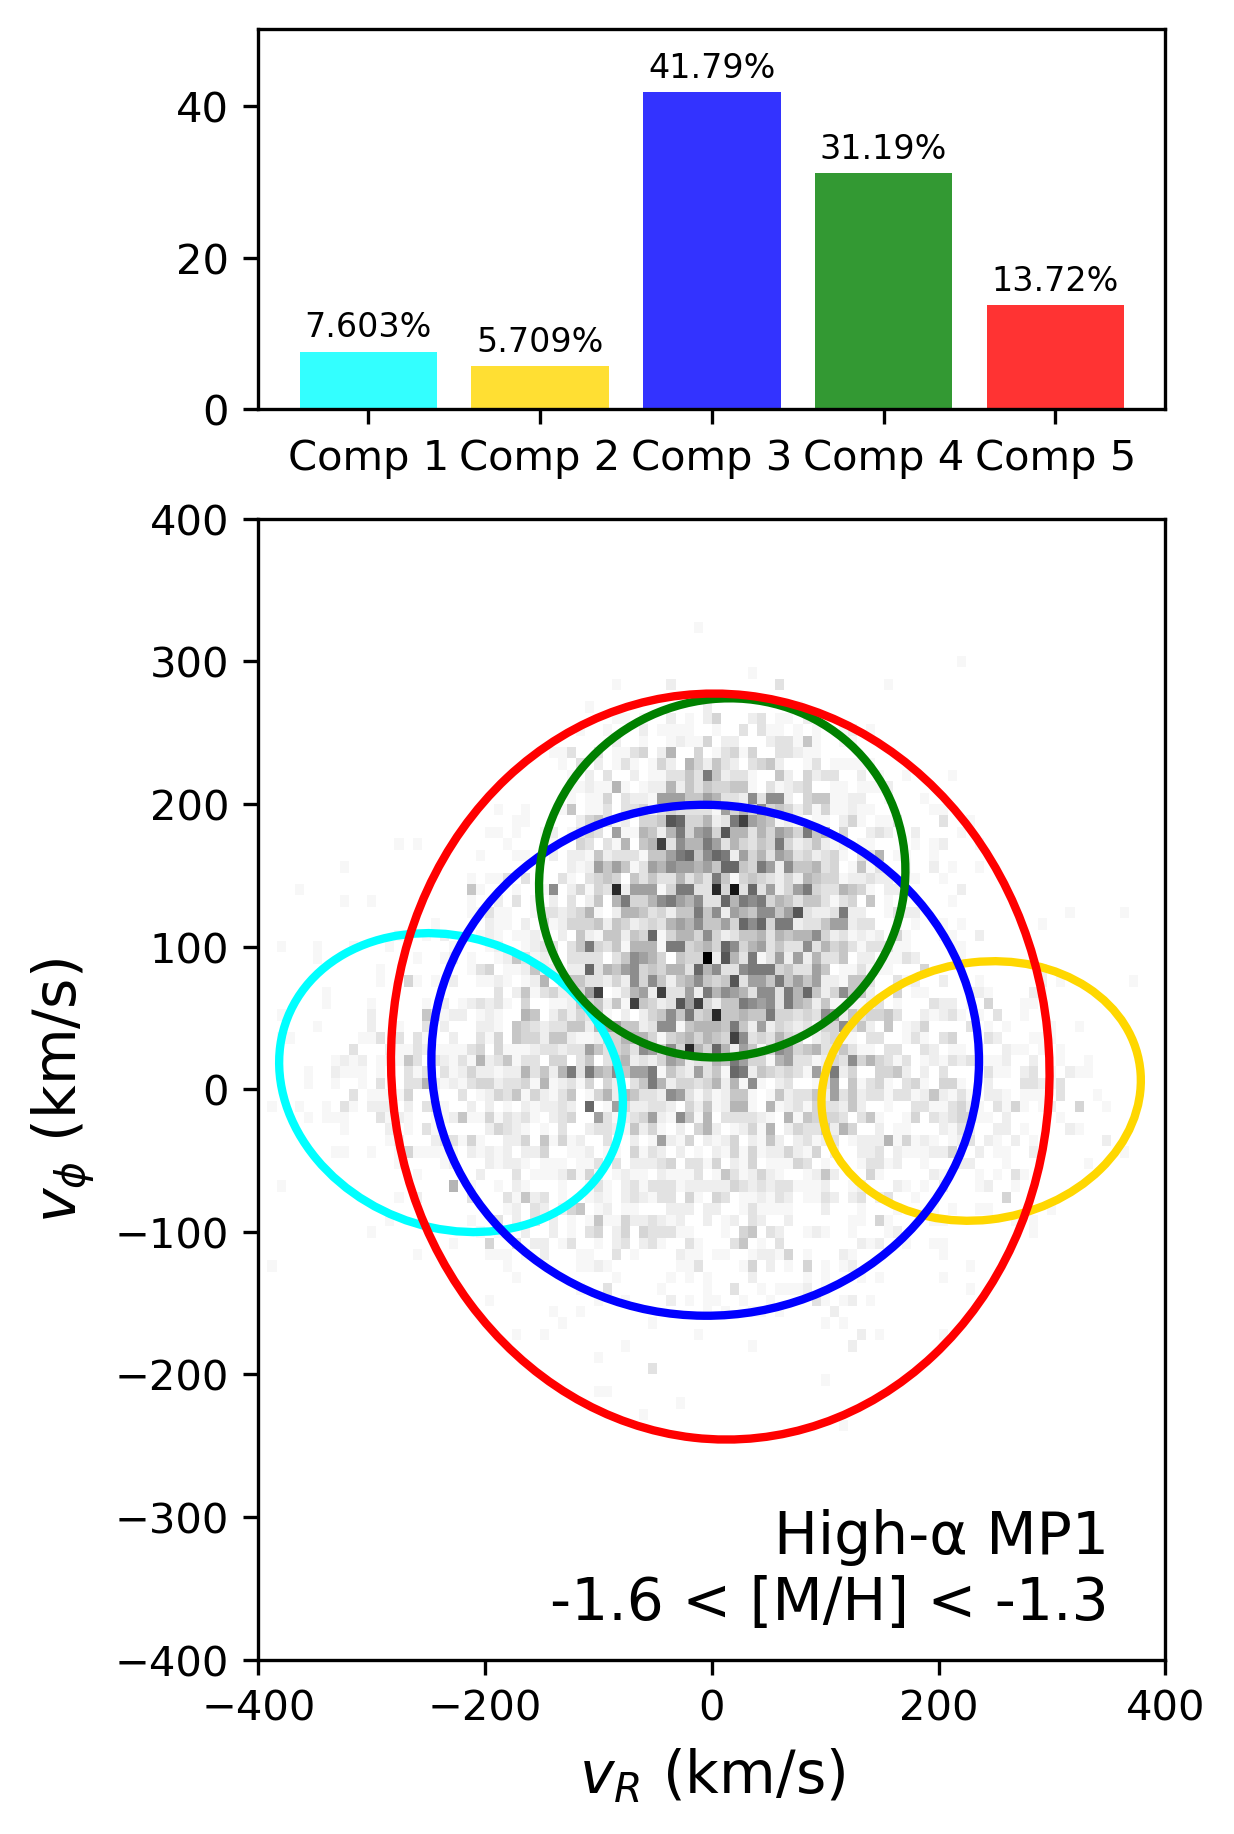
\includegraphics[width=\linewidth]{../figures/gmm_mp1_high_alpha_k5.png}
    \caption{\href{https://raw.githack.com/raunaq-rai/Disentangling-the-Milky-Way-using-GMM/main/figures/MP1\_high\_\_\_-1.6\%5BM\_H\%5D-1.3.html}{MP1 $\alpha_{\mathrm{high}}$}}
    \label{fig:mp1_hi}
  \end{subfigure}\hfill
  \begin{subfigure}[t]{0.24\linewidth}
    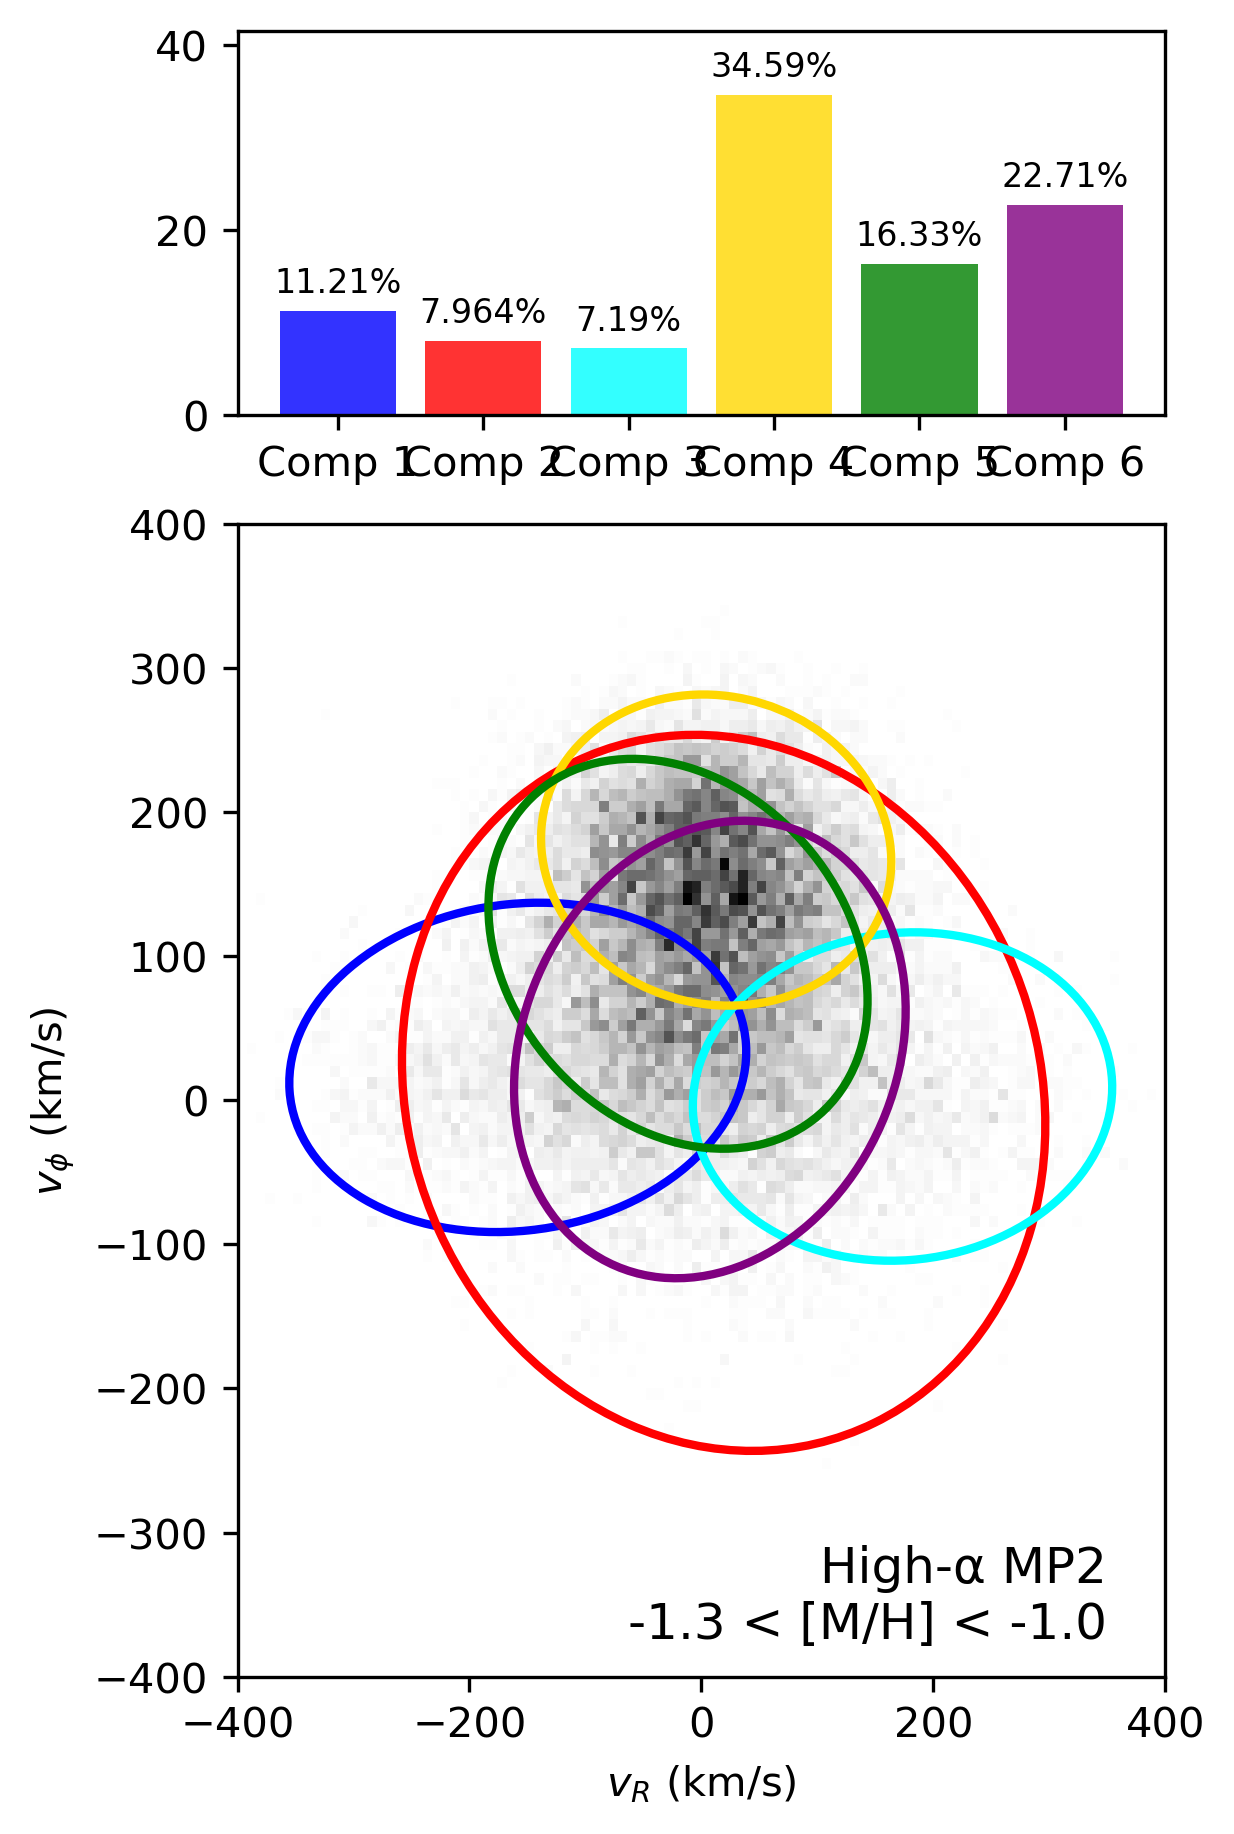
\includegraphics[width=\linewidth]{../figures/gmm_mp2_high_alpha_k6.png}
    \caption{\href{https://raw.githack.com/raunaq-rai/Disentangling-the-Milky-Way-using-GMM/main/figures/MP2\_high\_\_\_-1.3\%5BM\_H\%5D-1.0.html}{MP2 $\alpha_{\mathrm{high}}$}}
    \label{fig:mp2_hi}
  \end{subfigure}

  \vspace{0.5em}

  % Row 2: low-α (manual escapes)
  \begin{subfigure}[t]{0.24\linewidth}
    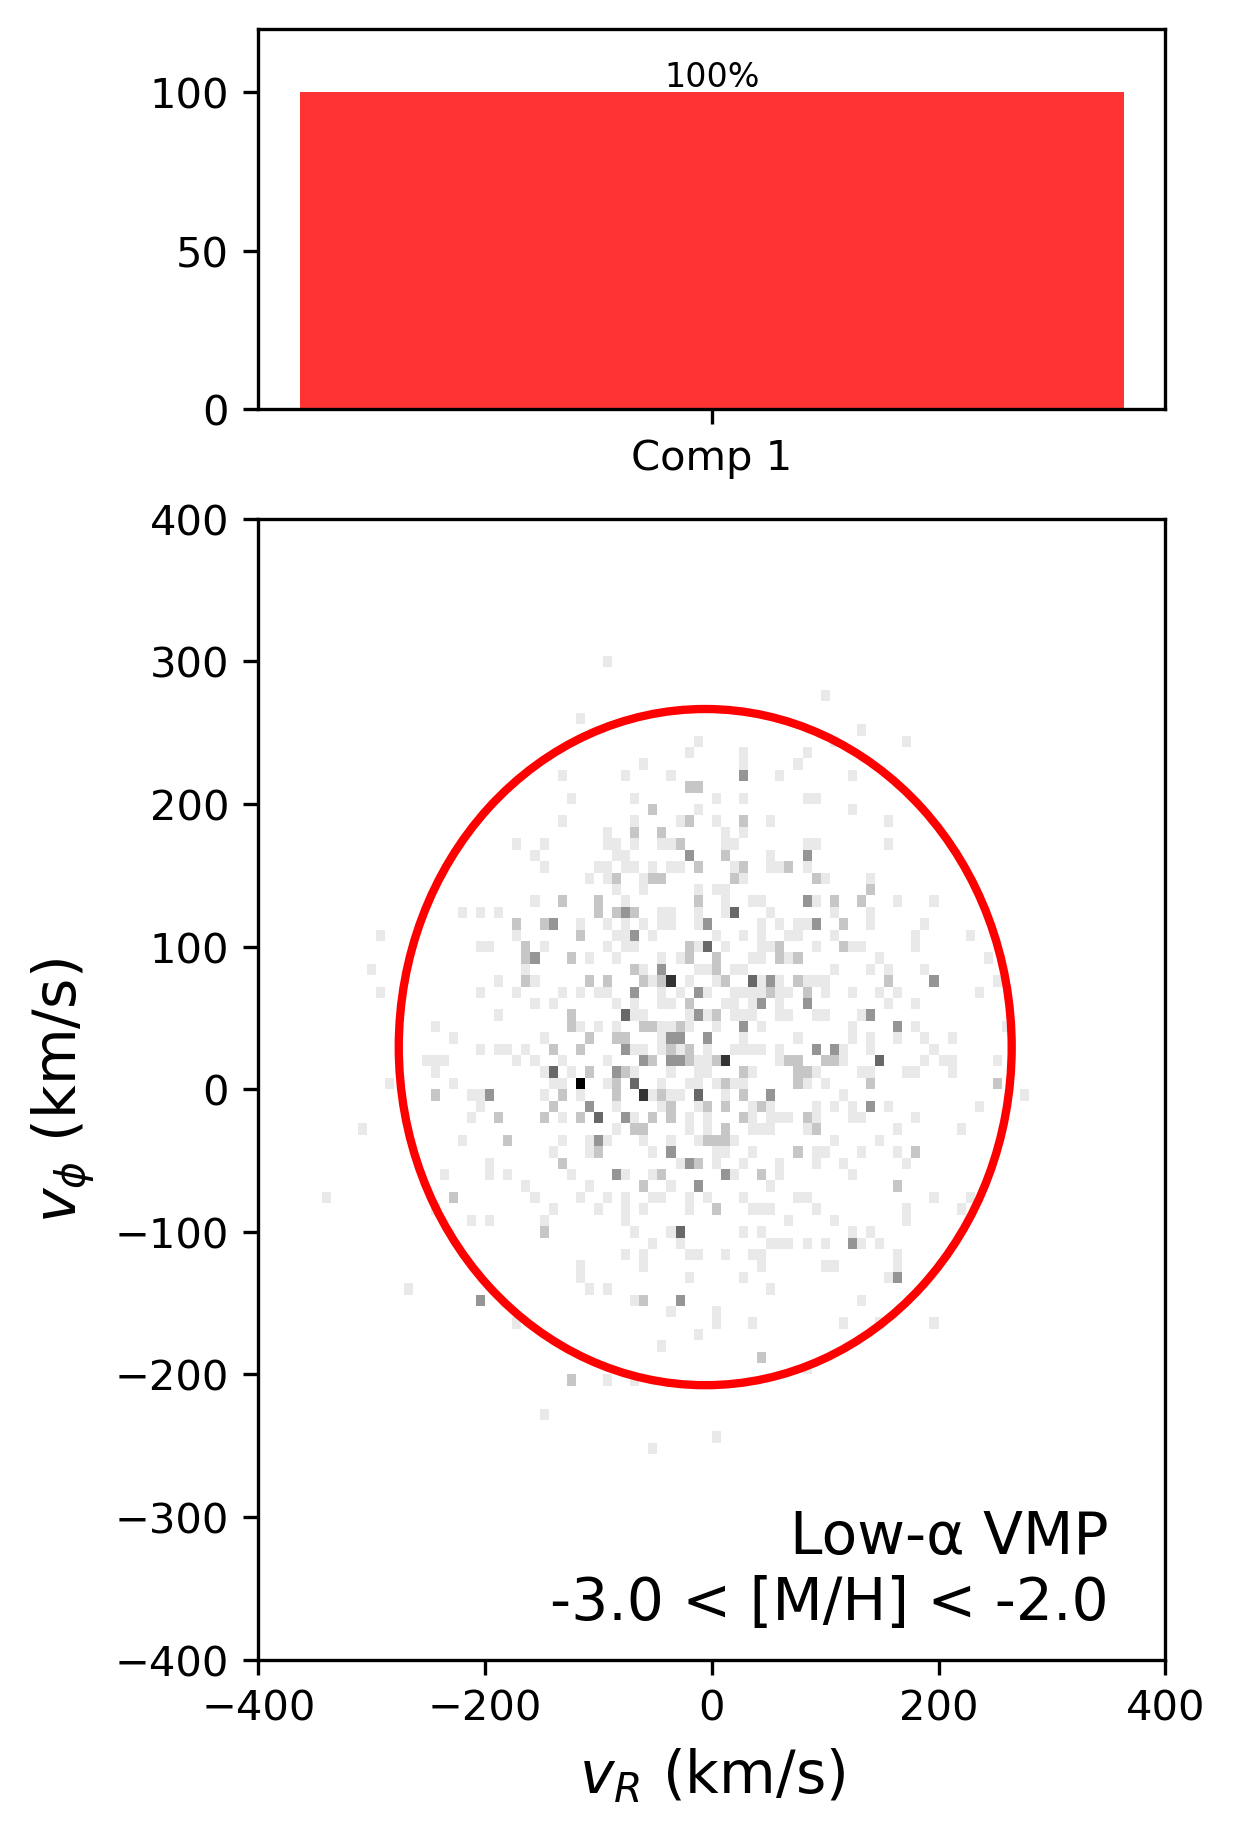
\includegraphics[width=\linewidth]{../figures/gmm_vmp_low_alpha_k1.png}
    \caption{\href{https://raw.githack.com/raunaq-rai/Disentangling-the-Milky-Way-using-GMM/main/figures/VMP\_low\_\_\_\_-3\%5BM\_H\%5D-2.html}{VMP $\alpha_{\mathrm{low}}$}}
    \label{fig:low_vmp}
  \end{subfigure}\hfill
  \begin{subfigure}[t]{0.24\linewidth}
    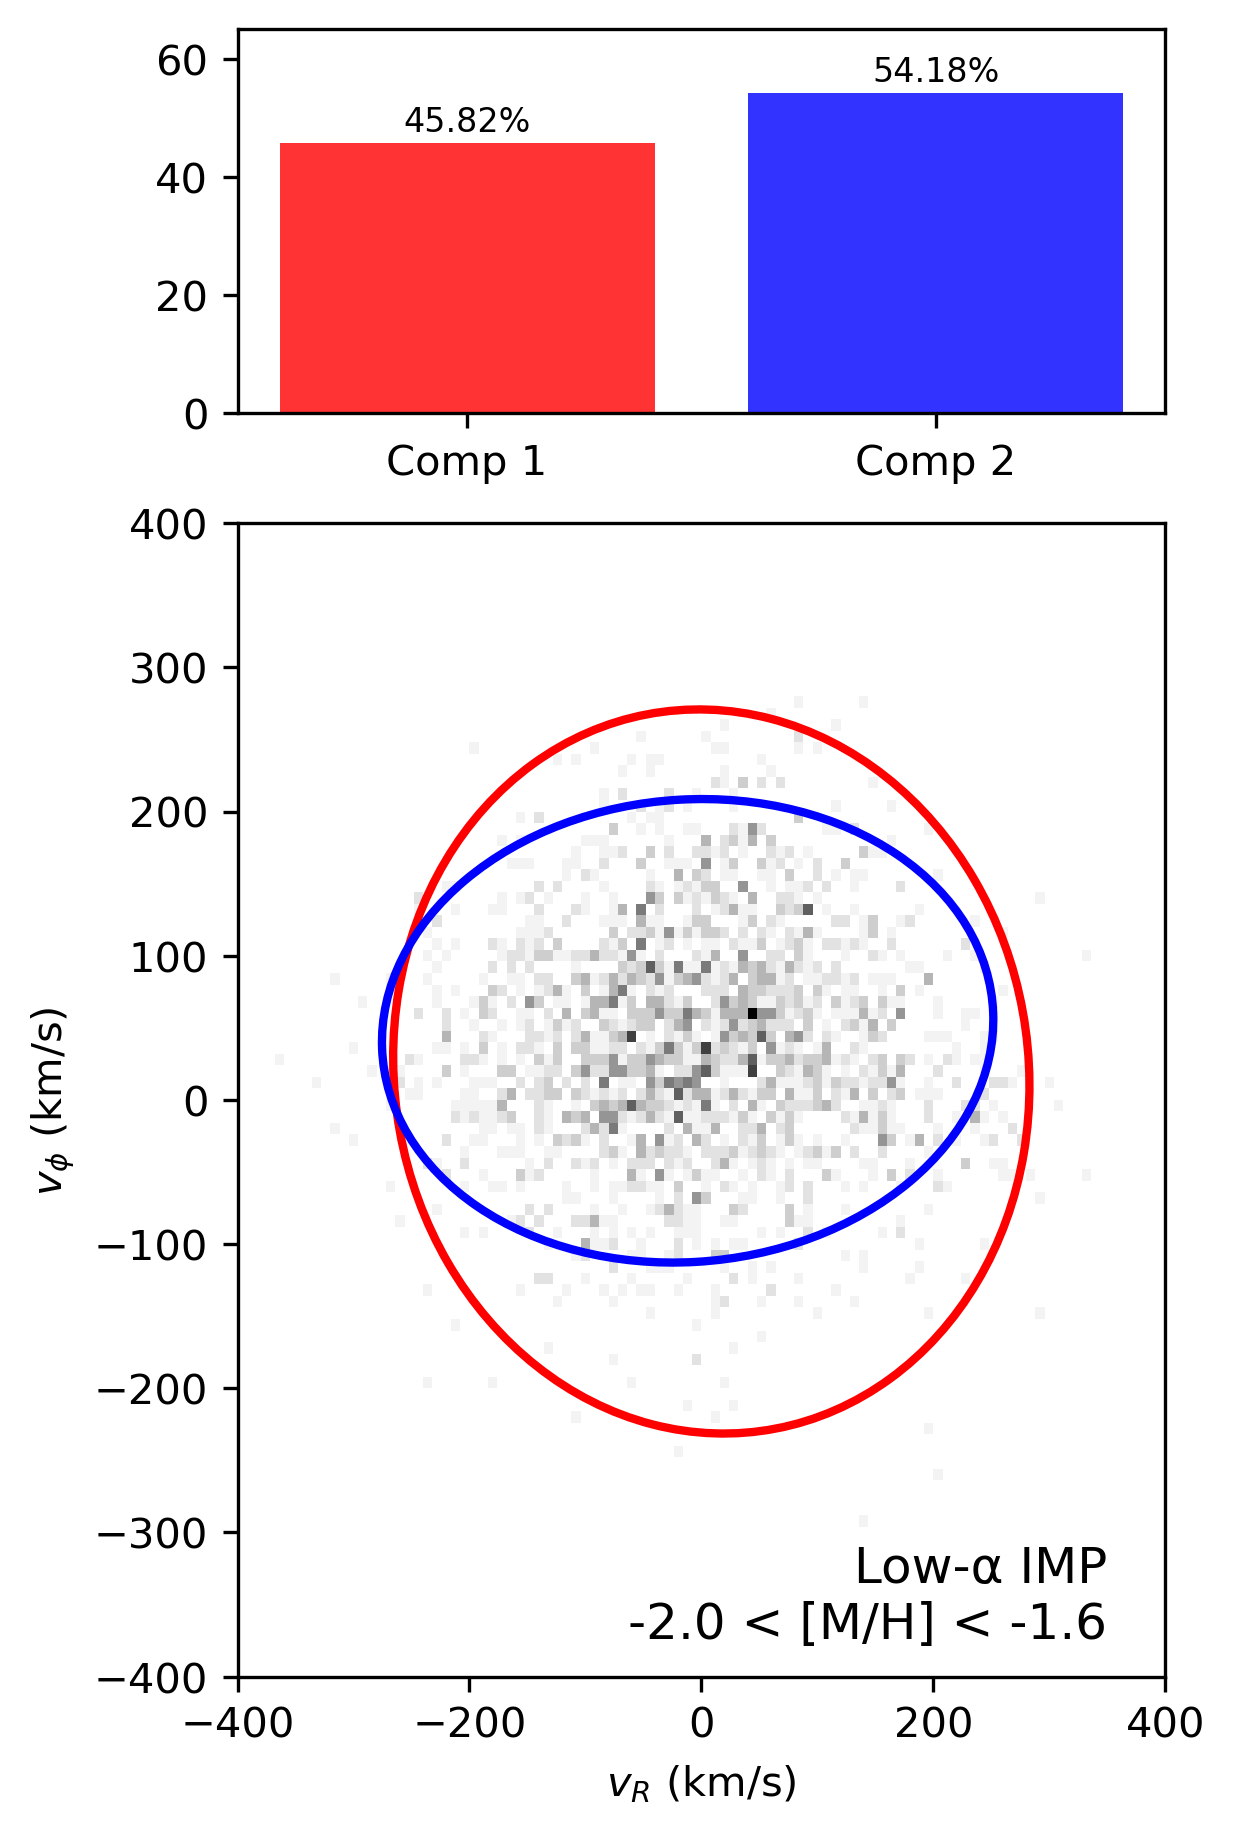
\includegraphics[width=\linewidth]{../figures/gmm_imp_low_alpha_k2.png}
    \caption{\href{https://raw.githack.com/raunaq-rai/Disentangling-the-Milky-Way-using-GMM/main/figures/IMP\_low\_\_\_\_-2\%5BM\_H\%5D-1.6.html}{IMP $\alpha_{\mathrm{low}}$}}
    \label{fig:low_imp}
  \end{subfigure}\hfill
  \begin{subfigure}[t]{0.24\linewidth}
    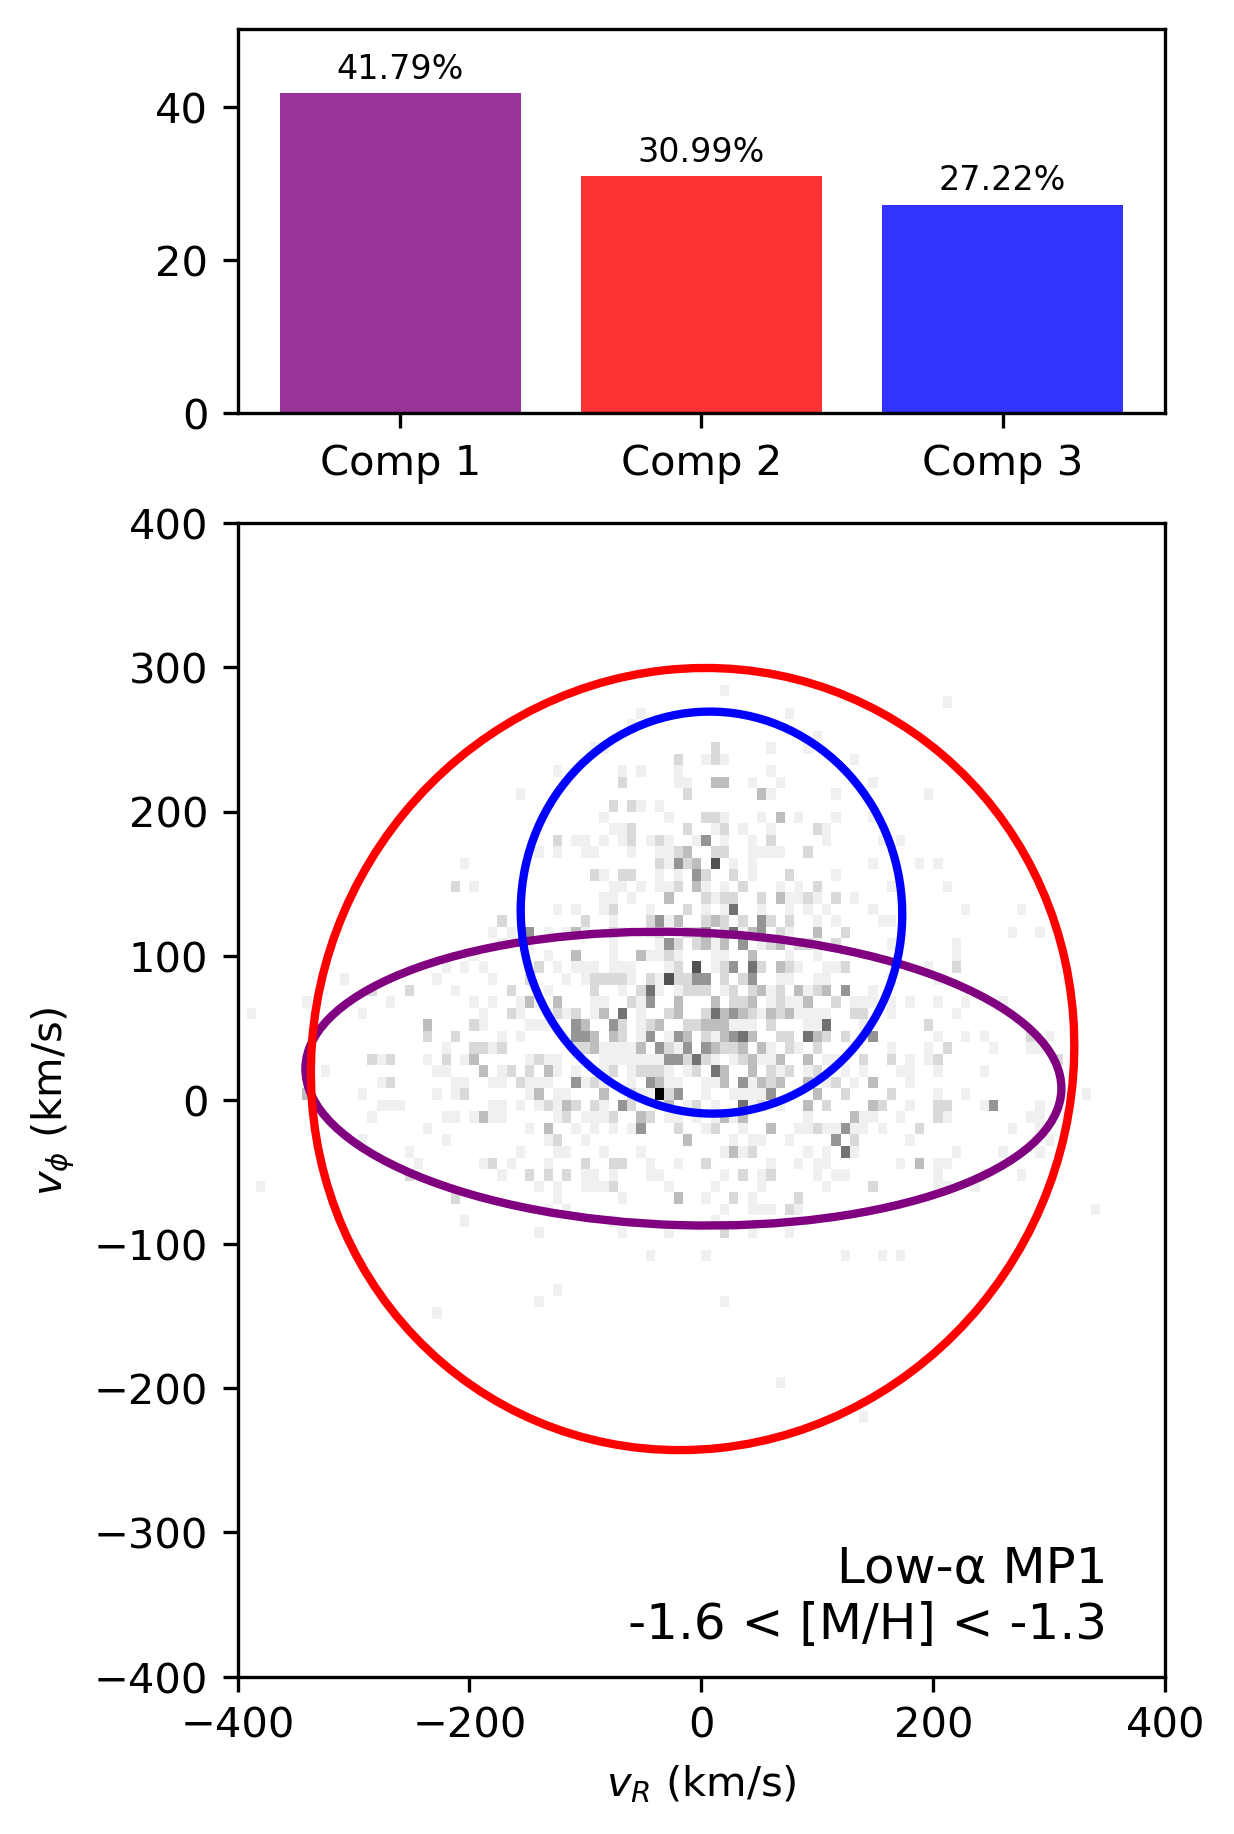
\includegraphics[width=\linewidth]{../figures/gmm_mp1_low_alpha_k4.png}
    \caption{\href{https://raw.githack.com/raunaq-rai/Disentangling-the-Milky-Way-using-GMM/main/figures/MP1\_low\_\_\_\_-1.6\%5BM\_H\%5D-1.3.html}{MP1 $\alpha_{\mathrm{low}}$}}
    \label{fig:low_mp1}
  \end{subfigure}\hfill
  \begin{subfigure}[t]{0.24\linewidth}
    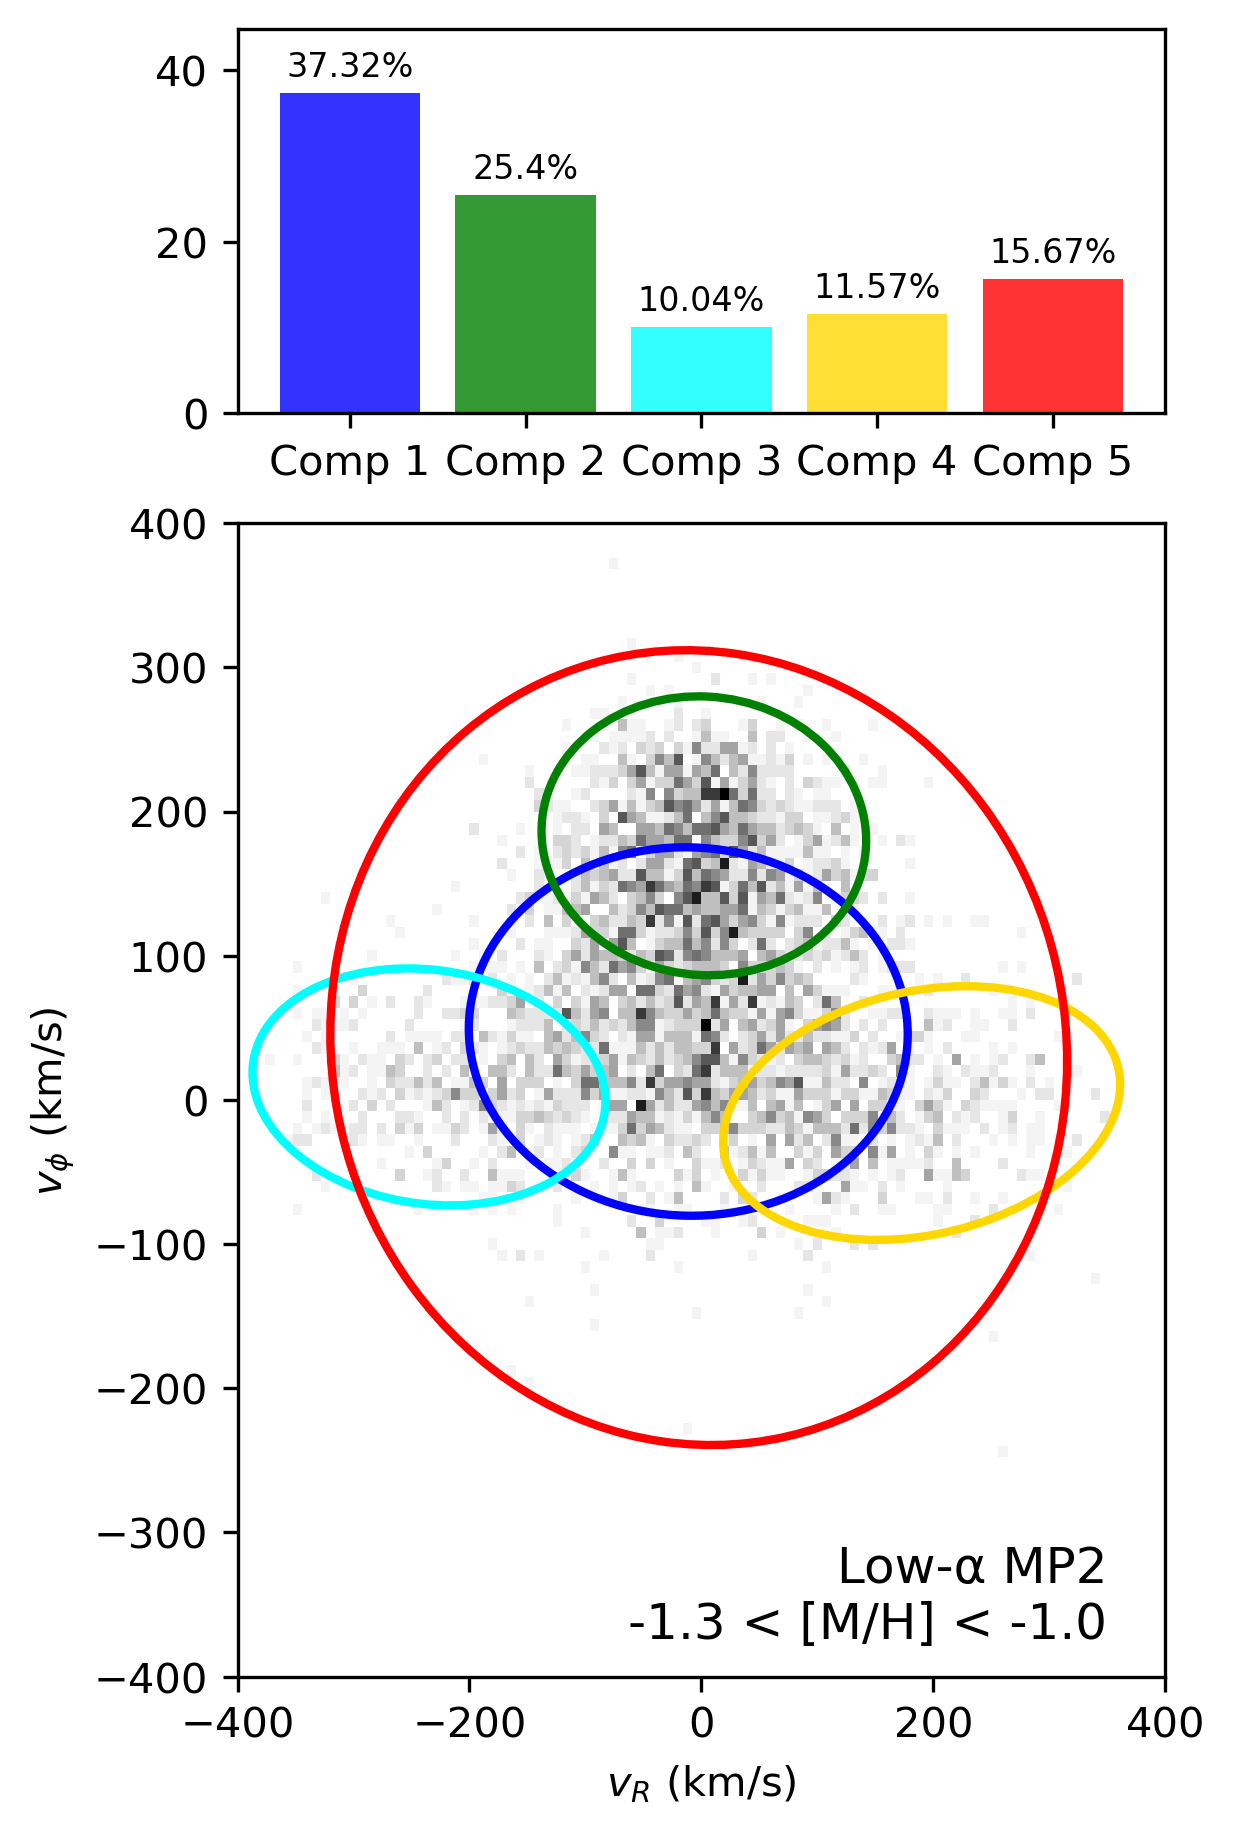
\includegraphics[width=\linewidth]{../figures/gmm_mp2_low_alpha_k6.png}
    \caption{\href{https://raw.githack.com/raunaq-rai/Disentangling-the-Milky-Way-using-GMM/main/figures/MP2\_low\_\_\_\_-1.3\%5BM\_H\%5D-1.0.html}{MP2 $\alpha_{\mathrm{low}}$}}
    \label{fig:low_mp2}
  \end{subfigure}


  \caption{XD-GMM decomposition across $\alpha$-sequences and metallicity bins. Top row: high-$\alpha$; bottom row: low-$\alpha$.}
  \label{fig:gmm_alpha_bins}
\end{figure}

% Chemistry-dependent disc growth
\paragraph{Chemistry-dependent disc growth (Fig.~\ref{fig:gmm_alpha_bins}).}

\begin{itemize}
  \item \textbf{High-$\alpha$ track:} Below $\mathrm{[M/H]}\lesssim -2$ the population is purely halo.  
        A thick-disc component appears at $-1.6 < [\mathrm{M/H}] < -1.3$ with 
        $V_{\rm rot}/\sigma_\phi \approx 2.4$ and grows steadily; by 
        $[\mathrm{M/H}]\approx -1.1$ it comprises $\sim$50\% of stars and 
        reaches $V_{\rm rot}/\sigma_\phi \approx 2.8$, indicating a gradual 
        thick-disc build-up.
  \item \textbf{Low-$\alpha$ track:} The distribution remains dispersion-dominated 
        until $-1.3 < [\mathrm{M/H}] < -1.0$, when a thick-disc component 
        ($\sim$25\%) emerges with $V_{\rm rot}/\sigma_\phi \approx 3.8$.  
        The high ratio suggests contamination by a colder thin disc and marks a 
        later, rapid disc-formation episode.
\end{itemize}

Taken together, the two sequences reveal a two-phase assembly: an early, 
slowly rotating high-$\alpha$ thick disc followed by a later, faster low-$\alpha$ 
disc that transitions to the present-day thin disc.


\section*{Recommendations and Next Steps}

\begin{itemize}
\item \textbf{Richer dynamical models.} Replace Gaussian mixtures with distribution-function or 
action-based models to capture non-Gaussian and asymmetric structures.  
\item \textbf{Tighter chemistry.} Improve $\alpha$–abundance precision (or use high-resolution 
follow-up) to reduce sequence cross-contamination, especially at low metallicity.  
\item \textbf{Explicit selection function.} Model Gaia’s magnitude and colour cuts to convert 
component weights into unbiased population fractions.  
\item \textbf{Chemical-abundance validation at low metallicity.} Gaia XP $\alpha$-element 
measurements become unreliable below $\mathrm{[M/H]}\!\approx\!-1.5$, so cross-match our 
sample with high-resolution spectroscopic surveys (e.g., APOGEE, GALAH) to secure precise 
abundances and verify whether the apparent GS/E signatures persist.
\end{itemize}

\section*{Conclusion and Research Impact}

Splitting Gaia DR3 red giants by $\alpha$ abundance reveals a \emph{two-phase} disc build-up:  
the high-$\alpha$ sequence gains rotational support at $\mathrm{[M/H]}\!\approx\!-1.6$, forming 
a thick disc that grows gradually, while the low-$\alpha$ sequence does not reach disc 
kinematics until $\mathrm{[M/H]}\!\approx\!-1.3$. This confirms that no metal-poor 
($\mathrm{[M/H]}\!<\!-2$) disc exists and clarifies the distinct evolutionary paths of 
the thick and thin discs.  

Coupling precise chemistry with full 3-D kinematics provides a template for forthcoming surveys 
(WEAVE, 4MOST, SDSS-V) to isolate, date and map Milky-Way disc components. Pinpointing the 
metallicity–$\alpha$ thresholds for disc formation tightens constraints on early star-formation, 
feedback and merger heating in disc galaxies, advancing our reconstruction of the Galaxy’s 
assembly history.  


\newpage{}

965 / 1000 words








\bibliographystyle{unsrt}  
\bibliography{references}

% End of two-column content
\end{multicols}



\end{document}
